% !TEX root = main.tex;

\documentclass[a4paper, oneside, 12pt]{report}
\usepackage[a4paper, inner=1.5cm, outer=3cm, top=2cm, bottom=3cm, bindingoffset=2cm]{geometry}

\usepackage[french]{babel}
% \usepackage{natbib}

% \usepackage[latin1]{inputenc}
\usepackage[T1]{fontenc}
\usepackage[utf8]{inputenc}
\usepackage{graphicx}
\usepackage{grffile}
\usepackage{verbatim}
\usepackage{float}
\usepackage{color}

\usepackage{colortbl}

\usepackage{titletoc}
%% enable styles for definitions
\usepackage{amsthm}
%% enable math
\usepackage{mathcomp}
\usepackage{amsmath}
\usepackage{amssymb}

\usepackage[export]{adjustbox}

\usepackage{mathrsfs}
\DeclareMathAlphabet{\mathpzc}{OT1}{pzc}{m}{it}
%% for tabs
\usepackage{booktabs}
\usepackage{array}
% \usepackage{standalone}
% \usepackage{tikz}
\usepackage{hyperref}
\usepackage{blindtext}
\usepackage{url}
\usepackage{titlesec}
\usepackage{lmodern}
\usepackage{fancyvrb}
\usepackage[justification=centering]{caption}
\usepackage{subcaption}
\usepackage[titletoc,toc,page]{appendix}

\usepackage[inline]{enumitem}
%% working with code
\usepackage{xcolor}
\usepackage{listings}
\definecolor{codegray}{rgb}{0.5,0.5,0.5}
\definecolor{backcolour}{rgb}{0.95,0.95,0.92}
\definecolor{darkblue}{rgb}{0.0,0.0,0.6}
\lstset{
  basicstyle=\ttfamily\footnotesize,
  breaklines=true,
  tabsize=2,
  frame=none,
  % caption=t,
  columns=fixed,
  fontadjust=true,
  basewidth=0.5em,
  stepnumber=1,
  numbers=left,
  numberstyle=\footnotesize\color{codegray},
  backgroundcolor=\color{backcolour},
  captionpos=b,
}

\lstdefinelanguage{XML} {
   % morestring=[b]",
   % moredelim=[s][\bfseries\color{darkblue}]{<}{\ },
   % moredelim=[s][\bfseries\color{darkblue}]{</}{>},
   % moredelim=[l][\bfseries\color{darkblue}]{/>},
   % moredelim=[l][\bfseries\color{darkblue}]{>},
   % morecomment=[s]{<?}{?>},
   % morecomment=[s]{<!--}{-->},
   % stringstyle=\color{black},
   % identifierstyle=\color{darkblue},
   % keywordstyle=\color{cyan},
   morekeywords={xmlns,version,type}% list your attributes here
}

\renewcommand{\appendixpagename}{Annexes}
\renewcommand{\appendixtocname}{Annexes}

\newlist{inlinelist}{enumerate*}{1}
\setlist*[inlinelist,1]{%
  label=(\roman*),
}

\newlist{enumerateRoman}{enumerate}{1}
\setlist*[enumerateRoman,1]{%
  label=(\roman*),
}

\setcounter{secnumdepth}{5}
\linespread{1.5}

\usepackage[acronym]{glossaries}

\usepackage[outdir=./]{epstopdf}
\makeglossaries
\author{TAOURIRIT Salah Eddine}
\title{composition des services web}

\date{\today\\version 0.3.1}
\begin{document}

% itemize style
\let\Item\item \newcommand{\head}[1]{\textnormal{\textbf{#1}}}

\newcommand\SpecialItem{\renewcommand\item[1][]{\Item[\hspace{0.5cm}\textbullet~\sffamily
    ##1]} }

\newcommand\SpecialItemI{\renewcommand\item[1][]{\Item[\textendash~\sffamily
    ##1]}}

% description style
\renewcommand{\descriptionlabel}[1]{\hspace{0.5cm}\textbullet~\textsf{#1}}
\renewcommand\enddescription{\endlist\global\let\item\Item}

% \renewcommand{\thesubsubsection}{\arabic{subsection}.\alph{subsubsection})}
% \renewcommand{\thesubsubsection}{\alph{subsubsection})}
\renewcommand{\thesubsubsection}{} % remore numbering
\newtheorem{mydef}{Definition}

% setup caption names
\captionsetup[figure]{name=Figure.}
\captionsetup[table]{name=Table.}

\maketitle

\setcounter{secnumdepth}{4}
\setcounter{tocdepth}{2}
\selectlanguage{french}

\pagenumbering{roman}
\tableofcontents
\newacronym{xml}{XML}{Extensible Markup Language}
\newacronym{xmls}{XML Schema}{XML Schema}
\newacronym{uri}{URI}{Uniform Resource Identifier}
\newacronym{url}{URL}{Uniform Resource Locator}
\newacronym{cgi}{CGI}{Common Gateway Interface}
\newacronym{soap}{SOAP}{Simple Object Access Protocol}
\newacronym{soa}{SOA}{Service-Oriented Architecture}
\newacronym{soc}{SOC}{Service-Oriented Computing}
\newacronym{wsdl}{WSDL}{Web Services Description Language}
\newacronym{uddi}{UDDI}{Universal Description Discovery and Integration}
\newacronym{w3c}{W3C}{The World Wide Web Consortium}
\newacronym{http}{HTTP}{Hypertext Transfer Protocol}
\newacronym{sawsdl}{SAWSDL}{Semantic Annotations for WSDL and XML Schema}
\newacronym{wsmo}{WSMO}{Web service modeling ontology}
\newacronym{wsml}{WSML}{web service modeling language}
\newacronym{swsf}{SWSF}{Semantic web services framework}
\newacronym{daml}{DAML}{the DARPA Agent Markup Language}
\newacronym{darpa}{DARPA}{Defence Advanced Research Projects Agency}
\newacronym{bpel}{BPEL}{Business Process Execution Language}
\newacronym{ws-bpel}{WS-BPEL}{Web Service Business Process Execution Language}
\newacronym{bpel4ws}{BPEL4WS}{Business Process Execution Language for Web Services}
\newacronym{xlang}{XLANG}{XML Business Process Language}
\newacronym{wsfl}{WSFL}{Web Services Flow Language}
\newacronym{wsci}{WSCI}{Web Service Choreography Interface}
\newacronym{ws-cdl}{WS-CDL}{Web Services Choreography Description Language}
\newacronym{wsmf}{WSMF}{The Web Service Modeling Framework}
\newacronym{qos}{QoS}{Quality of service}
\newacronym{mdo}{MDO}{Model driven engineering}
\newacronym{sws}{SWS}{synthesized Web services}
\newacronym{uml}{UML}{Unified Modeling Language}
\newacronym{ccs}{CCS}{Calculus of Communicating Systems}
\newacronym{csp}{CSP}{Communicating Sequential Processes}
\newacronym{json}{JSON}{JavaScript Object Notation}
\newacronym{nosql}{NoSQL}{Not Only SQL}
\newacronym{SGBD}{SGBD}{Système De Gestion Des Bases de Données}
\newacronym{SGBDR}{SGBDR}{Système De Gestion Des Bases de Données Relationnelles}
\newacronym{DSL}{DSL}{Domain Specific Language}
\newacronym{sparql}{SPARQL}{SPARQL Protocol and RDF Query Language}
\newacronym{rdf}{RDF}{Resource Description Framework}
\newacronym{rdf/xml}{RDF/XML}{XML syntax for RDF}
\newacronym{rdfs}{RDFS}{Resource Description Framework Schema}
\newacronym{cap}{CAP}{Consistency, Availability and Partition Tolerance}
\newacronym{acid}{ACID}{(Atomicity, Consistency, Isolation, Durability)}
\newacronym{rest}{REST}{Representational State Transfer}
\newacronym{wsfl}{WSFL}{Web Services Flow Language}
\newacronym{crud}{CRUD}{Create, Read, Update, and Delete}
\newacronym{gd}{GD}{Graphe de Dépendance}
\newacronym{html}{HTML}{HyperText Markup Language}
\newacronym{owl}{OWL}{The Web Ontology Language}
\newacronym{oil}{OIL}{Ontology Inference Layer}
\newacronym{isbn}{ISBN}{International Standard Book Number}
\printglossaries\
\listoffigures
\listoftables

\newpage
\pagenumbering{arabic}

\input{chapters/introduction}
\part{Étude bibliographique}
%% !TEX root = ../main.tex
\chapter{Services Web}
\label{ch:web-service}

\section*{Introduction}
\addcontentsline{toc}{section}{Introduction} \markboth{INTRODUCTION}{}

Plusieurs paradigmes de développement de logiciels ont été proposés
pour satisfaire le besoin de la \textit{réutilisation}, le paradigme
orienté service (\acrshort{soa}) représente aujourd'hui une approche
largement adoptée pour le développement des systèmes d'information
distribués sur \textit{Internet}. En effet, il adopte les avantages
des autres paradigmes comme l'orientaté objet et l'orienté composant,
tels que \textit{l'encapsulation}, \textit{la modularité}, \textit{le
  couplage faible} et \textit{l'interopérabilité}. Le paradigme
\acrshort{soa} possède plusieurs implémentations telles que
\textit{DCOM}~\cite{frank1997dcom}, \textsc{CORBA}
\cite{vinoski1997corba},\textsc{RPC}~\cite{bloomer1992power} et
\acrshort{rest}~\cite{fielding2000architectural}. Dans ce travail,
nous nous intéressons uniquement aux services Web basés sur la
spécification \acrshort{soap} (\textit{SOAP-based Web services}), qui
représentent la concrétisation la plus répandue dans
l'industrie.\bigskip

Ce chapitre établit une étude du fondement théorique de notre travail
à savoir les notions de base du paradigme service Web. Nous commençons
par introduire le concept de (\acrshort{soc}) et \acrshort{soa}, ainsi
que les services Web~\ref{sec:ws-definitions}, leurs architectures et
leurs infrastructures, puis nous présentons un socle technologique
très répandu pour la mise en œuvre d'une telle
architecture~\ref{sec:ws-standards}. Ensuite nous nous focalisons sur
les modèles de description des services tout en mettant l'accent sur
l'enrichissement sémantique de la représentation des services
Web~\ref{sec:ws-description}. La dernière partie de ce
chapitre~\ref{sec:ws-discovery} est consacrée à la présentation de
quelques approches de découverte des services Web rencontrées dans la
littérature.

\newpage
\section{Définitions}
\label{sec:ws-definitions}
L'objectif de cette section est d'introduire les concepts et
terminologies associés au paradigme \textit{orientaté service}. Dans
la première section~\ref{sec:soc}, nous allons définir le
\textit{``Service oriented computing''} (\acrshort{soc}) comme un
modèle émergent de développement rapide des applications distribuées
dans les environnements hétérogènes. Nous présentons ensuite
l'architecture orientée service pour réaliser le \acrshort{soc}
(section~\ref{sec:soa}). Dans la section~\ref{sec:ws-def}, nous nous
focalisons sur les services Web en présentant quelques définitions et
caractéristiques rencontrées dans la littérature.

  \subsection{L'approche orientée service}
  \label{sec:soc}
  L'approche orientée service (\acrshort{soc}) est un paradigme
  informatique qui vise la construction d'applications distribuées
  interopérables et à faible coût utilisant des entités logicielles
  appelées \emph{services}.\bigskip

  Selon Papazoglou~\cite{papazoglou2003service}: \textit{``Les
    services sont des éléments logiciels auto-descriptifs, définis
    indépendamment de toute plate-forme ou technologie''}\bigskip

  Selon le style architectural \acrshort{soc}, les applications sont
  construites à partir de services autonomes, auto-descriptifs et
  faiblement couplés, exposant leurs fonctionnalités sous forme
  d'interfaces bien définies en s'abstrayant complètement de leurs
  implémentations. Grâce à leurs descriptions publiées, ces services
  peuvent être recherchés et ensuite invoqués par des utilisateurs ou
  d'autres services clients, permettant une meilleure collaboration
  entre plusieurs entreprises de différents domaines.\medskip

  \subsection{Architecture orientée services}
  \label{sec:soa}
  Pour réaliser le style architectural présenté précédemment
  (\acrshort{soc}), il faut mettre en place un environnement
  d'intégration et d'exécution des services. L'architecture orientée
  services (\acrshort{soa}) a été donc proposée afin de promouvoir
  l'interopérabilité et l'extensibilité des services dans
  l'ensemble.\bigskip

  Selon \textit{OASIS}\footnote{\url{https://www.oasis-open.org}}:
  \textit{``L'architecture orientée services est un paradigme
    permettant d'organiser et d'utiliser des fonctionnalités
    distribuées pouvant être de domaines variés. Cela fournit un moyen
    uniforme d'offrir, de découvrir, d'interagir et d'utiliser ces
    fonctionnalités pour produire le résultat désiré avec des
    préconditions et des buts mesurables.''}\bigskip

  Une architecture à base de
  services~\cite{gottschalk2002introduction} est constitué d'un
  fournisseur de service \textit{(service provider)}, un annuaire des
  services \textit{(service registry)}, et un client de service
  \textit{(service requester)}.

  \input{figs/ws-basic-arch.tex}

  La figure~\ref{fig:ws-basic-arch} montre comment ces trois rôles
  interagissent:

  \renewcommand{\descriptionlabel}[1]{\hspace{0.5cm}\textbullet~\textsf{#1}}
  \begin{description}
  \item[Le fournisseur]: Un prestataire de services fournit
    l'interface pour le service Web et l'implémentation de
    l'application.

  \item[L'annuaire]: Un registre de service est une façon dont les
    services Web sont officiellement publiés. Le registre de service
    est basée sur la spécification \acrshort{uddi} et reflète des
    informations sur les services fournis par le fournisseur.

  \item[Le client]: Un client d'un service est le consommateur d'un
    service Web, il utilise le registre de service pour obtenir des
    informations et pour pouvoir accéder à un service Web.
  \end{description}
  \enddescription

  Pour qu'une application puisse profite des services Web, trois
  comportements doivent avoir lieu: \textit{la publication} de
  descriptions des services, \textit{la découverte} de ces
  descriptions et enfin \textit{l'invocation} des services:

  \renewcommand{\descriptionlabel}[1]{\hspace{0.5cm}\textbullet~\textsf{#1}}
  \begin{description}
  \item[Publier]: Pour être accessible, une description de service
    doit être publiée afin que le client puisse la trouver.

  \item[Découvrir]: Lors de la découverte d'un service, le client
    interroge un annuaire (ou un registre) de services pour une
    catégorie requise de services et récupère une description
    détaillée.

  \item[Invoquer (bind)]: le client peut ainsi invoquer une
    fonctionnalité particulière dans le service cible utilisant les
    détails de liaison dans la description du service pour le
    localiser, contacter et l'appeler.
  \end{description}
  \enddescription

  La \acrshort{soa} n'est pas liée à une technologie particulière. En
  effet, il existe une multitude d'implémentations techniques de cette
  architecture, y compris les services Web~\cite{WSA},
  \acrshort{rest}~\cite{fielding2000architectural},
  \textsc{CORBA}~\cite{vinoski1997corba}, etc. Dans notre travail nous
  nous limitons aux services Web (ou plus clairement
  \textit{SOAP-based web services}).

  \subsection{Services Web}
  \label{sec:ws-def}
  Les services Web sont l'approche la plus populaire pour mettre en
  œuvre une architecture \acrshort{soa}. Le terme service Web qualifie
  tout service disponible par Internet, qui utilise un format standard
  (généralement \acrshort{xml} ou \acrshort{json}) d'échange de
  messages, et qui n'est pas lié à un système d'exploitation ou un
  langage de programmation particulier.\\

  À l'origine, la technologie des services Web a été initiée par
  IBM~\cite{kreger2001web} et Microsoft, puis en partie standardisée
  par le consortium du
  \acrshort{w3c}~\footnote{\url{http://www.w3.org/}}, l'organisme
  chargé de standardiser les spécifications techniques du Web.\medskip

  D'après Curbera \emph{et al.}~\cite{curbera2001web}:\bigskip

  \textit{``Un service Web est une application réseau capable
    d'interagir par le moyen des standards et des protocoles via des
    interfaces bien spécifiées, dans lesquelles il est décrit
    utilisant un langage de description fonctionnel
    standardisé.''}\bigskip

  Selon Cubera \emph{el al.}, un service Web est vu principalement
  comme une application réseau accessible à partir d'autres
  applications. Cette définition est très ouverte dans le sens ou elle
  permet de considérer toute application identifiée par une
  \acrshort{url} comme un service Web, ce qui est pas le cas pour les
  scripts \acrshort{cgi} ou les applications \textsc{CORBA} par
  exemple.\medskip

  \acrshort{w3c} fournit une définition plus spécifique aux services
  Web~\cite{WSA}:\bigskip

  \textit{``Un service Web est un système conçu pour permettre
    l'interopérabilité des applications à travers un réseau.  Il est
    caractérisé par un format de description
    interprétable/compréhensible automatiquement par la machine,
    D'autres systèmes peuvent intéragir avec le Service Web selon la
    manière prescrite dans sa description et en utilisant des messages
    SOAP, généralement transmis via le protocole HTTP et sérialisés en
    XML ou en d'autres standards du Web.''} \bigskip

  Cette définition souligne les caractéristiques suivantes des
  services Web~\cite{fremantle2002enterprise}:

  \renewcommand{\descriptionlabel}[1]{\hspace{0.5cm}\textbullet~\textsf{#1}}
  \begin{description}
  \item[Basés sur des protocoles Internet]: L'utilisation de
    \acrshort{http} pour le transport des informations permet de
    traverser les contrôles d'accès dans un environnement hétérogène.

  \item[Interopérables]: Le standard
    \acrshort{soap}~\cite{box2000simple} définit comme étant un
    protocole destiné à l'échange de messages structurés véhiculés
    généralement sur \acrshort{http} et sérialisé en \acrshort{w3c},
    permettant ainsi le support pour l'interopérabilité.

  \item[Basés sur XML]: Le métalangage de balises \acrshort{w3c}
    \textit{eXtensible Markup Language} est un standard Web ouvert par
    \textsc{W3C}~\cite{bray1998extensible} qui offre un cadre standard
    pour la définition de documents interprétables par des machines.
  \end{description}
  \enddescription

  M. P. Papazoglou~\cite{papazoglou2003service} apporte une autre
  définition détaillée de services Web (traduction par
  \cite{driss2011approche}):\bigskip

  \textit{``Les services Web sont des éléments auto-descriptifs et
    indépendants des plates-formes permettent la composition faible
    coût d’applications distribuées. Les services Web effectuent des
    fonctions allant de simples requêtes aux processus métiers
    complexes. Les services Web permettent aux organisations d'exposer
    leurs programmes résultats sur Internet (ou sur un intranet) en
    utilisant des langages (basés sur XML) et des protocoles
    standardisés et de les mettre en œuvre via une interface
    auto-descriptive basée sur des formats standardisés et
    ouverts.''}\bigskip

  L'approche de service Web vise essentiellement quatre objectifs
  fondamentaux expliquant son grand succès \cite{driss2011approche}:

  \renewcommand{\descriptionlabel}[1]{\hspace{0.5cm}\textbullet~\textsf{#1}}
  \begin{description}
  \item [L'interopérabilité:] l'interopérabilité permet à des
    applications écrites dans des langages de programmation différents
    et s'exécutant sur des plates-formes différentes pour communiquer
    entre elles.

  \item [le couplage faible:] Le couplage est une métrique indiquant
    le niveau d'interaction entre deux ou plusieurs composants
    logiciels. Deux composants sont dits couplés s'ils échangent de
    l'information.

  \item [La réutilisation:] L'avantage de la réutilisation est qu'elle
    permet de réduire le coût de développement en réutilisant
    des composants déjà existants.

  \item [La découverte et la composition automatique:] La découverte
    et la composition sont des étapes importantes qui permettent la
    réutilisation des services. En effet il faudra être en mesure de
    trouver et de composer un service afin de pouvoir en faire
    usage. En exploitant les technologies offertes par
    \textit{Internet} et en utilisant un ensemble de standards pour la
    publication, la recherche et la composition.
  \end{description}
  \enddescription

  Techniquement, un service Web est donc une entité logicielle offrant
  une ou plusieurs fonctionnalités allant des plus simples aux plus
  complexes. Ces entités sont \emph{décrites}, \emph{publiées},
  \emph{découvertes}, \emph{invoquées} et \emph{composées} grâce à
  l'utilisation de Web (avec \acrshort{http}) comme infrastructure de
  communication ainsi que de formats de données standardisés basés sur
  \acrshort{xml}.

\section{Standards de services Web}
\label{sec:ws-standards}
Les services Web sont construits autour de standards qui sont
\acrshort{soap}, \acrshort{wsdl} et \acrshort{uddi}, assurant
respectivement leur \emph{communication}, leur \emph{description} et
leur \emph{découverte}. La figure~\ref{fig:ws-standards-relationships}
illustre les relations sous-jacentes entre ces spécifications et la
contribution de chacune d'entre elles dans le processus de mise en oeuvre
d'une architecture à base de services Web.\bigskip

%!TEX root = ../main.tex
\begin{figure}[h]
    \centering
    \includegraphics[width=0.8\textwidth]{figs/ws-standards-relationships.eps}
    \caption{Les relations entre les standards de services
      Web.~\cite{erl2004service}}
    \label{fig:ws-standards-relationships}
\end{figure}

%%% Local Variables:
%%% mode: latex
%%% TeX-master: "../main"
%%% End:


Dans la suite de cette section, nous présentons brièvement ces trois
spécifications, leurs origines, structures et fonctionnalités de base.

\newpage
  \subsection{Communication: SOAP}
  \label{sec:soap}
  Développé par IBM et Microsoft \cite{box2000simple}, le langage
  \acrshort{soap} est une recommandation \acrshort{w3c}
  \cite{mitra2003soap} qui le définit comme étant un protocole destiné
  à l'échange de messages structurés, permettant d'invoquer des
  applications sur des réseaux distribués. \acrshort{soap} est basé
  sur \acrshort{xml} pour mettre en place un mécanisme valable
  d'échange de données indépendant du modèle de programmation de
  l'application et du système d'exploitation.\medskip

  Un message \acrshort{soap} est un document \acrshort{xml} constitué
  d'une enveloppe \acrshort{soap} obligatoire, d'une en-tête
  \acrshort{soap} facultative et d'un corps \acrshort{soap}
  obligatoire (voir la
  figure~\ref{fig:soap-message-structure}):\bigskip

  \input{figs/soap-message-structure}\bigskip

  \renewcommand{\descriptionlabel}[1]{\hspace{0.5cm}\textbullet~\textsf{#1}}
  \begin{description}
  \item[Enveloppe \texttt{<Enveloppe>}]: L'élément racine du message
    \acrshort{soap}, définissant le contexte du message, son
    destinataire et son contenu, il englobe l'en-tête et le corps.

  \item[En-tête \texttt{<Header>}]: Un mécanisme générique permettant
    d'ajouter des fonctions à un message \acrshort{soap} d'une manière
    modulaire sans accord préalable entre les parties en
    communication. Des exemples d'extension qui peuvent être
    implémentés comme des en-têtes peuvent être des authentifications,
    des transactions, des paiements.

  \item[Corps \texttt{<Body>}]: Contient les informations obligatoires
    destinées à l'ultime destinataire du message, il sert comme un
    conteneur pour les informations mandataires à l'intention du
    récepteur du message. \acrshort{soap} définit un élément pour le
    corps, qui est l'élément \texttt{<Fault>} utilisé pour rapporter
    les erreurs.
  \end{description}
  \enddescription

  \subsection{Description: WSDL}
  \label{sec:wsdl}
  Le langage de description de services Web \acrshort{wsdl}
  \cite{christensen2001web, chinnici2007web} est une recommandation du
  \acrshort{w3c}, maintenant dans sa deuxième version.
  \acrshort{wsdl} est basé sur \acrshort{xml} pour décrire les
  fonctions opérationnelles du service Web. La description
  \acrshort{wsdl} est composée d'une interface et des
  implémentations. L'interface est une définition abstraite et
  réutilisable du service qui peut être référencée par plusieurs
  implémentations.\medskip

  \acrshort{wsdl} fournit un modèle ainsi qu'un langage basé sur
  \acrshort{xml} de description de services Web. Un fichier
  \acrshort{wsdl} comprend une description des fonctionnalités d'un
  service, mais il ne se préoccupe pas de l'implantation de celles-ci.
  Il contient aussi des informations concernant la localisation du
  service, ainsi que les données et les protocoles à utiliser pour
  l'invoquer. En pratique, le document
  \acrshort{wsdl}\footnote{\url{http://www.w3.org/TR/wsdl20/}} est un
  document \acrshort{xml} qui se divise en deux parties
  \cite{elie2010}:\medskip

  \input{figs/wsdl-document-structure.tex}\medskip

  \SpecialItem
  \begin{itemize}
  \item La définition \textbf{abstraite} de l'interface du service
    avec les opérations supportées par le service Web, ainsi que leurs
    paramètres et les types de données.

  \item La définition \textbf{concrète} de l'accès au service avec la
    localisation par une adresse réseau du fournisseur de service et
    les protocoles spécifiques d'accès.\medskip
  \end{itemize}
  \enddescription

  La partie abstraite d'un document \acrshort{wsdl} contient deux
  sous-parties:\medskip

  \renewcommand{\descriptionlabel}[1]{\hspace{0.5cm}\textbullet~\texttt{#1}}
  \begin{description}
  \item[<Types>]: décrit sous la forme d'un schéma \acrshort{xml} les
    types de données échangées entre le client et le fournisseur de
    service.

  \item[<Interface>]: Les interfaces \acrshort{wsdl} offrent une
    manière abstraite pour décrire la fonctionnalité du service, ils
    définissent les opérations (éléments \texttt{<operation>}) en terme de
    paramètres d'entrée et de sortie sous forme d'un modèle
    d'échange de message \textit{(message exchange
      pattern)}. \acrshort{wsdl} contient huit modèles de messages
    prédéfinis, mais on peut facilement définir de nouveaux.\medskip
  \end{description}
  \enddescription

  La définition concrète d'un document \acrshort{wsdl} est constituée
  de:\medskip

  \renewcommand{\descriptionlabel}[1]{\hspace{0.5cm}\textbullet~\texttt{#1}}
  \begin{description}
  \item[<Binding>]: L'élément \texttt{Binding} reprend les opérations
    de l'élément \texttt{<Interface>} et leurs associe un protocole de
    transfert et des spécifications des formats de données de message.

  \item[<Service>]: Cet élément définit la localisation du service Web
    décrit. Pour chaque interface décrite, un élément service lui est
    associée. Le sous-élément \texttt{<endpoint>} définit un port
    d'accès en référençant l'élément \texttt{<binding>} associé et en
    déclarant l'\acrshort{url} localisant le service (avec l'attribut
    \texttt{<address>}).
  \end{description}

  \newpage
  \subsection{Découverte: UDDI}
  \label{sec:uddi}
  \acrshort{uddi} \cite{clement2004uddi} est une standardisation pour
  la publication et la découverte de services Web, initialement conçue
  et spécifiée par le Consortium de standards
  OASIS\footnote{\url{https://www.oasis-open.org}}, il est le résultat
  d'un accord d'un ensemble d'industriels
  Ariba\footnote{\url{http://www.ariba.com/}}, IBM, Microsoft, etc en
  vue de devenir le registre standard de la technologie de services
  Web.\medskip

  \acrshort{uddi} complète les technologies basiques de services Web
  par la création d'un \textit{annuaire} permettant de localiser
  les services web recherchés sur le réseau. Les services référencés
  dans \acrshort{uddi} sont accessibles par l'intermédiaire du
  protocole de communication \acrshort{soap}, et la publication des
  informations concernant les fournisseurs et les services doit être
  spécifiée en \acrshort{xml} afin que la recherche et l'utilisation
  soient faites de manière \textit{dynamique} et
  \textit{automatique}.\medskip

  Un registre \acrshort{uddi} peut appartenir à un domaine public
  comme \textit{Internet} ou tout autre réseau accessible à un nombre
  non limité d'utilisateurs, comme il peut appartenir à un domaine
  restreint comme l'\textit{Intranet} d'une entreprise ou d'un groupe
  d'entreprises. Les données stockées dans l'\acrshort{uddi} sont
  structurées (en \acrshort{xml}) et organisées en trois parties
  connues:\medskip

  \renewcommand{\descriptionlabel}[1]{\hspace{0.5cm}\textbullet~\textsf{#1}}
  \begin{description}
    \item[Pages blanches]: fournissent des descriptions générales sur
      les fournisseurs de services à savoir le nom de l'entreprise qui
      fournit le service, son identificateur commercial, ses adresses,
      etc.

    \item[Pages jaunes]: comportent des descriptions détaillées sur
      les fournisseurs de services catalogués dans les pages blanches
      d'une façon taxonomique (selon secteurs d'activités par
      exemple).

    \item[Pages vertes]: fournissent des informations techniques sur
      les services Web catalogués. Ces informations incluent la
      description du service, les adresses \textsc{URL}, du processus
      de son utilisation et des protocoles utilisés pour son
      invocation.
  \end{description}

\section{Description sémantique de services Web}
\label{sec:ws-description}
La description de services Web est une étape primordiale dans
le cycle de vie d'une application à base de services. Elle permet
d'une manière claire et structurée au fournisseur de services
de communiquer au client les spécifications pour invoquer un service
Web. Le \acrshort{w3c} propose de décrire syntaxiquement les services
Web en utilisant le standard \acrshort{wsdl} \cite{christensen2001web,
  chinnici2007web} et de les publier dans l'annuaire \acrshort{uddi}
\cite{clement2004uddi}. Malgré les améliorations apportées au standard
\acrshort{wsdl} dans sa deuxième version \cite{chinnici2007web}, la
description des services reste insuffisante lors des processus de
sélection, découverte, et composition. Pour pallier cette
difficulté, plusieurs approches \cite{sivashanmugam2003adding,
  mcilraith2001semantic, mcilraith2003bringing, fensel2002web,
  paolucci2002semantic} proposent de rajouter une couche sémantique au
dessus de \acrshort{wsdl} complétant la description syntaxique par des
précisions sémantiques. Les services Web enrichis par des métadonnées
supplémentaires exprimant leur sémantique sont appelés \textit{les
services Web sémantiques}.\medskip

\input{figs/www-to-sws.tex}

Les services Web sémantiques sont le résultat de la convergence de la
technologie de services Web et du Web sémantique (illustré dans La
figure\ref{fig:www-to-sws}), cette combinaison des technologies
va permettre de:

\begin{itemize}\renewcommand\labelitemi{--}
\item Automatiser l'invocation et l'exécution du service Web par un
  service client ou par un agent.

\item Automatiser la découverte dee services.

\item La composition automatique des services Web.
\end{itemize}
\enddescription

Dans cette section, nous allons présenter les diverses approches
sémantiques visant à préciser la description d'un service en insistant
sur les approches d'annotation sémantique
(\ref{sec:semantic-annotation}) et sur les ontologies de services
(\ref{sec:ontologies-services}). La notion du Web sémantique est
abordée brièvement dans l'annexe~\ref{annexe:semantic-web}.

  \subsection{Annotations sémantiques}
  \label{sec:semantic-annotation}
  L'annotation sémantique consiste à enrichir et à compléter la
  description d'un service. Elle établit des correspondances entre des
  éléments de la description et des concepts d'un ensemble
  d'ontologies de références. Une ontologie de référence permet de
  représenter un domaine par des structures interprétables par une
  machine. Deux modèles principaux suivent l'approche d'annotation
  sémantique, à savoir \textsc{WSDL-S} et \acrshort{sawsdl}
  \cite{elie2010}.

    \subsubsection{WSDL-S}
    \textsc{WSDL-S} \cite{akkiraju2005web} est le résultat d'un
    travail collaboratif entre IBM, le laboratoire LSDSI et
    l'université de Geogia. La spécification est devenue une
    recommandation\footnote{\url{http://www.w3.org/Submission/WSDL-S/}}
    \acrshort{w3c} depuis 2005. Son objectif principal est de fournir
    un processus d'annotation sémantique compatible avec les
    technologies existantes. Pratiquement, le méta-modèle
    \textsc{WSDL-S} repose sur les éléments extensibles du modèle
    \acrshort{wsdl} introduits dans sa deuxième version en rajoutant
    trois éléments majeurs \texttt{<category>},
    \texttt{<precondition>} et \texttt{<effect>}, et deux attributs,
    \texttt{modelReference} et \texttt{schemaMapping}.\medskip

    \renewcommand{\descriptionlabel}[1]{\hspace{0.5cm}\textbullet~\texttt{#1}}
    \begin{description}
    \item [<category>:] est un sous-élément de \texttt{<portType>}. Il
      précise la catégorie d'un service lors de la publication dans un
      annuaire ou registre.

    \item [<precondition>:] sous-élément de \texttt{<operation>},
      indique les préconditions à vérifier pour que l'opération
      s'exécute comme prévu.

    \item [<effects>:] sous-élément de \texttt{<operation>}, indique
      les effets de l'exécution de l'opération.

    \item [modelreference:] Un attribut qui peut être ajouté à élément
      dans une grammaire \acrshort{xml} et aux éléments
      \texttt{<category>}, \texttt{<precondition>} et
      \texttt{<effects>}. Il indique une association avec un élément
      correspondant dans une ontologie donnée.

    \item [schemamapping:] Un attribut peut être ajouté à un élément
      dans une grammaire \acrshort{xml}. Il permet de décrire les
      correspondances entre la grammaire annotée et les ontologies de
      référence.
    \end{description}
    \enddescription
    \bigskip

    Les éléments permettent de rajouter des informations
    qui n'étaient pas prises en compte dans \acrshort{wsdl} comme
    \emph{les préconditions} et \emph{les effets} d'une opération,
    tandis que les attributs permettent de référencer des concepts
    dans des ontologies de référence, ces préconditions et effets.

    \subsubsection{SAWSDL}
    \acrshort{sawsdl} \cite{kopecky2007sawsdl} est un langage
    d'annotation sémantique de description de services Web qui hérite
    de \textsc{WSDL-S}. Issu d'une initiative du groupe de travail
    d'annotations sémantiques pour
    \acrshort{wsdl}\footnote{\url{http://www.w3.org/TR/sawsdl/}} et
    soumis au \acrshort{w3c} en 2007, \acrshort{sawsdl} définit un
    mécanisme pour annoter sémantiquement les interfaces et les
    opérations \acrshort{wsdl}, ainsi que les types \textit{``XML
      schema''} en les reliant à des concepts dans une
    ontologie.\medskip

    Cette annotation repose sur la définition d'attributs étendant le
    standard de description en référençant des ontologies
    préexistantes. Le mécanisme d'annotation de \acrshort{sawsdl} est
    indépendant de tout langage de représentation
    \cite{lopez2008selection} d'ontologies.\medskip

    \acrshort{sawsdl} propose trois sortes d'annotations sémantiques
    pour référencer des concepts de modèles définis à l'extérieur du
    document \acrshort{wsdl}, une pour identifier le concept
    sémantique (représentée par l'attribut \texttt{modelReference}) et
    deux autres (\texttt{liftingSchemaMapping} et
    \texttt{loweringSchemaMapping}) pour spécifier la correspondance
    (\emph{Mapping}) entre les données sémantiques et les éléments
    \acrshort{xml}:\bigskip

    \renewcommand{\descriptionlabel}[1]{\hspace{0.5cm}\textbullet~\texttt{#1}}
    \begin{description}
    \item [modelReference:] Il permet d'associer un composant
      \acrshort{wsdl} ou une instance\acrshort{xml} schema à un concept
      d'une ontologie.

    \item [liftingSchemaMapping:] Il définit comment un élément
      \acrshort{xml} peut être transformé en une donnée conforme
      à un certain modèle sémantique.

    \item [loweringSchemaMapping:] Dans le sens inverse que le
      précédent, cet attribut définit comment les données dans un
      modèle sémantique sont transformées en instances \acrshort{xml}.
    \end{description}
    \enddescription

  \subsection{Ontologies de services}
  \label{sec:ontologies-services}
  Une ontologie de services saisit les différents aspects liés à la
  description de services et leurs utilisations à travers un ensemble
  de concepts, de propriétés et de relations entre eux
  \cite{elie2010}. Deux modèles d'ontologies de services sont décrits
  dans cette sous-section \textsc{OWL-S} et \acrshort{wsmo}.

    \subsubsection{WSMO}
    \label{sec:wsmo}
    \acrshort{wsmo} \cite{de2005web} est un modèle conceptuel basé sur
    la spécification \acrshort{wsmf} \cite{fensel2002web}
    (voir~\ref{sec:wsmf}) pour la description des divers aspects liés
    aux services Web sémantiques. Le but de \acrshort{wsmo} est
    d'automatiser le cycle de vie de services web (publication,
    sélection, découverte, composition, etc.) afin de résoudre le
    problème de l'intégration de services Web en définissant une
    technologie cohérente pour la description de services Web
    sémantique.\medskip

    Pour formaliser \acrshort{wsmo}, le groupe de travail a mis au
    point le langage de modélisation \acrshort{wsml} \cite{de2006web}
    et a défini plusieurs variantes de celui-ci, chacune basée sur
    différents formalismes.\medskip

    \acrshort{wsmo} est constitué de quatre composants: les services
    web, les buts, les ontologies et les médiateurs. Ce modèle permet
    de réaliser un couplage faible entre les services web en utilisant
    un ensemble de médiateurs. Ces derniers assurent les tâches
    d'intégration d'ontologies, de découverte de services, de
    composition, etc.

    \newpage
    \subsubsection{OWL-S}
    \label{sec:owl-s-1}
    \textsc{OWL-S} \cite{martin2004owl} désigné par \textsc{DAML-S}
    \cite{ankolekar2002daml} dans les versions antérieures, est un
    langage issue des travaux de
    \acrshort{darpa}\footnote{\url{http://www.darpa.mil/}} et son
    programme
    \acrshort{daml}\footnote{\url{http://www.daml.org/services/}} en
    collaboration avec des chercheurs de plusieurs universités et
    organisations. Il a été intégré au consortium \acrshort{w3c} en
    2004 au sein du groupe d'intérêt sur les services Web sémantiques,
    lors de la recommandation du langage \textsc{OWL}
    \cite{horrocks2002daml+oil, mcguinness2004owl}. Ankolekar \emph{et
      al.}  \cite{ankolekar2002daml} présentent une ontologie pour les
    services web dans le but d'automatiser la \emph{découverte},
    \emph{l'invocation}, la \emph{composition} et la
    \emph{surveillance} de l'exécution des services
    \cite{mcilraith2003bringing}, les auteurs reprennent la notion de
    classes d'\textsc{OWL} et proposent l'ontologie
    \textsc{OWL-S}.\bigskip

    \input{figs/owls.tex}

    L'objectif principal de ces recherches est d'établir une
    plate-forme dans laquelle les descriptions de services Web sont
    partagées en utilisant une ontologie standard, constituée d'un
    ensembles de classes de base et des propriétés pour résoudre les
    ambiguïtés et de rendre la description d'un service compréhensible
    par la machine.\bigskip

    la figure~\ref{fig:owl-s} décrit la structure tripartie d'une
    ontologie \textsc{OWL-S}. Elle est composée de trois
    sous-ontologies: un \emph{service profil}, un \emph{service model}
    et un \emph{service grounding}:

    \renewcommand{\descriptionlabel}[1]{\hspace{0.5cm}\textbullet~\texttt{#1}}
    \begin{description}
    \item[ServiceProfile]: il offre une description informelle des
      fonctionnalités rendues par le service (\verb|serviceName|,
      \verb|textDescription|) et des informations concernant son
      fournisseur (\verb|contactInformation|). D'un autre côté, il
      spécifie des fonctionnalités offertes par le service (
      comportement fonctionnel) en terme de transformation
      d'informations dénotées par les \textit{entrées/sorties}
      \textsc{(I/O)} (\verb|hasInput|, \verb|hasOutput|) et de
      changement d'état après l'exécution du service dénoté par les
      \textit{préconditions/effets} \textsc{(P/E)}
      (\verb|hasPrecondition|, \verb|hasResult|).\medskip

      Du point de vue découverte et composition, Le
      \verb|ServiceProfile| est la partie la plus importante de la
      définition du service \textsc{OWL-S}.

    \item[ServiceModel]: il décrit le fonctionnement du service en
      indiquant comment les résultats sont produits étape par étape
      précisant la façon qu'un client peut interagir avec le service
      afin d'atteindre sa fonctionnalité. Ceci est fait en exprimant
      la transformation de données avec \textit{Entrées/Sorties}
      \textsc{(I/O)} et la transformation de l'état avec
      \textit{pré-conditions/effets} \textsc{(P/E)}.\medskip

      le \verb|ServiceProfile| est généralement considéré comme un
      sous-ensemble du \verb|ServiceModel|, contenant uniquement
      l'information nécessaire pour annoncer le service Web pour une
      découverte ultérieure.

    \item[ServiceGrounding]: Permet de spécifier les détails d'accès
      au service en précisant le protocole, le format des messages, la
      sérialisation et l'adressage. Il représente une correspondance
      \textit{(mapping)} entre la définition abstraite d'un processus
      \textsc{OWL-S} décrivant le service et la définition
      \textsc{WSDL} concrète des éléments nécessaires pour interagir
      avec le service.
    \end{description}
    \enddescription

    Le \verb|ServiceProfile| fournit éventuellement d'autres
    informations supplémentaires sur le service comme la qualité qu'il
    assure en terme de temps de réponse et de coût, une classification
    possible d'un service (\verb|serviceCategory|), et un paramètre
    générique \verb|serviceParameter|.

\newpage
\section{Découverte de services web}
\label{sec:ws-discovery}
La découverte de services Web présente un axe de recherche très
important. Divers mécanismes de découverte ont été proposés dans la
littérature et plusieurs définitions sont attribuées à ce
concept. Booth \textit{el al.} \cite{booth2004web} décrivent le
processus de découverte comme étant l'acte de \textit{``localisation
  d'une description compréhensible par la machine d'un service
  éventuellement inconnu au préalable écrivant certains critères
  fonctionnels.''}

\input{figs/ws-discovery-with-matching.tex}

Essentiellement, un processus de découverte de service web s'effectue
en deux phases principales (illustrés dans la
figure~\ref{fig:ws-discovery-with-matching}). Premièrement, un module
de mise en correspondance (\textit{Matching}) renvoie tous les
services Web candidats selon le degré de similitude entre les services
disponibles et les exigences spécifiées par la requête (aspect
fonctionnel). La deuxième étape consiste à sélectionner et invoquer le
service le plus satisfaisant (aspect \textit{non-fonctionnel}).

Plusieurs critères peuvent être utilisés pour catégoriser les
approches de découverte des services \cite{mohebbi2010comparative,
  elie2010, bitar2014cbr4wsd}):

  \begin{enumerate}
  \item la localisation de services
    (\textit{centralisation/décentralisation} des annuaires).
  \item Le degré d'automatisation du processus de la découverte.
  \item le principe de l'algorithme de \textit{Matching}.
  \end{enumerate}

  Cette section vise à présenter les différentes approches de
  découverte des services Web proposées dans la littérature. Ces
  modèles ont été classés selon les critères déjà mentionnés, à savoir
  la localisation~\ref{sec:ws-localisation} (centralisée, distribuée),
  le degré d'automatisation du
  processus~\ref{sec:ws-desc:manual-vs-auto} (manuel, automatique), et
  le niveau de \textit{Matching}~\ref{sec:ws-matching} (syntaxique ou
  sémantique).

\subsection{Localisation de services}
\label{sec:ws-localisation}
La découverte consiste principalement à localiser les descriptions de
services répondant à une requête cliente. Les approches de
localisation de services récurrentes dans la littérature sont classées
en deux catégories, à savoir les approches centralisées et les
approches décentralisées ou distribuées \cite{garofalakis2004web}.

    \subsubsection{Approches centralisées}
    \label{sec:ws-localisation-centr}
    Les premières versions d'\acrshort{uddi} \cite{clement2004uddi}
    (présenté dans~\ref{sec:uddi}) reposent sur une approche
    \textit{centralisée} de publication et découverte de services Web.
    Le registre \acrshort{uddi} définit un modèle de représentation
    des données et des métadonnées nécessaires à la publication, il
    s'appuie sur \textit{un seul annuaire} qui peut être géré par un
    module de mise en correspondances \textit{(matchmaker)}.

    \subsubsection{Approches décentralisées}
    \label{sec:ws-localisation-distr}
    Les approches décentralisées de découverte de services
    \cite{rompothong2003query, sivashanmugam2004discovery,
      paolucci2003using, schmidt2004peer, verma2005meteor,
      sahin2005spider} consistent à mettre en place une
    \textit{fédération} d'annuaires \acrshort{uddi} agissant comme une
    couche d'abstraction reliant plusieurs instances d'annuaires. La
    plupart des approches distribuées sont basées sur des systèmes
    pair-à-pair (\textit{peer to peer}) incluant
    \cite{schmidt2004peer, verma2005meteor, sahin2005spider}.

    La dernière version d'\acrshort{uddi}
    \cite{oasis2005specification} (\textit{3.0.2}) reprend le principe
    d'une fédération d'annuaires et décrit un annuaire \acrshort{uddi}
    comme un ensemble de nœuds \textit{(UDDI nodes)} tel que chaque
    nœud fait partie d'un seul annuaire et possède une copie répliquée
    de schéma global de la fédération. Les nœuds d'un annuaire
    collaborent pour gérer un ensemble de structures de données
    \acrshort{uddi} pour permettre une meilleure gestion des requêtes.

  \subsection{Découverte manuelle/automatique}
  \label{sec:ws-desc:manual-vs-auto}
  le degré d'intervention de l'utilisateur dans la découverte varie
  selon la richesse sémantique de la description du service. Nous
  pouvons distinguer les approches manuelles et semi-automatiques
  d'une part, et les approches automatiques d'une autre part
  \cite{elie2010,garofalakis2004web}.

    \subsubsection{Approches manuelles et semi-automatiques}
    Dans une découverte manuelle, le client utilise un service de
    découverte pour localiser et sélectionner manuellement une
    description de service qui répond à certains critères
    fonctionnels. La recherche de descriptions dans cette approche est
    souvent basée sur une simple comparaison syntaxique entre les mots
    clés de la requête et les descriptions de services disponibles, ce
    qui nécessite l'intervention de l'utilisateur pour vérifier la
    pertinence et la fiabilité des résultats de la recherche et
    sélectionner le service Web qui répond au mieux à ses exigences.

    \subsubsection{Approches automatiques}
    La découverte automatique de services qui répond à un besoin donné
    est considéré comme une étape cruciale vers l'intégration
    dynamique et évolutive de services Web. On entend par découverte
    automatique la possibilité de localiser automatiquement un service
    Web qui répond à des besoins particuliers. Différentes approches
    ont été proposées pour réaliser la découverte dynamique de
    services ( \cite{paolucci2002semantic, bernstein2002discovering,
      mandell2003bottom,
      benatallah2005automating,keller2005automatic}).\medskip

    Dans \cite{mandell2003bottom} les auteurs présentent une approche
    d'automatisation de la découverte de services modélisés en
    \acrshort{bpel} (voir~\ref{sec:bpel}) dans le but d'une
    composition plus dynamique. Les auteurs proposent d'étendre la
    description \textsc{BPEL} par l'intégration d'une description
    sémantique \textsc{OWL-S} (voir~\ref{sec:owl-s}) de type
    \textit{service profile} et la mise en place d'un module de
    \textit{Matching} sémantique équipé par un raisonneur
    automatique. Autrement, Keller \textit{et al}
    \cite{keller2005automatic} étudient un modèle de localisation
    automatique de services Web décrits via le modèle \acrshort{wsmo}.

  \subsection{Matching de services Web}
  \label{sec:ws-matching}
  Le \textit{Matching} (ou le \textit{Matchmaking}) de services Web
  est défini comme un processus qui nécessite un annuaire de services
  pour prendre une requête en entrée, et de retourner les services les
  plus pertinents qui peuvent satisfaire les exigences spécifiées dans
  cette requête \cite{li2004software}. Cette opération nécessite la
  recherche de similarités indiquant le degré de rapprochement entre
  les paramètres descriptifs \textit{fonctionnels} (les paramètres
  \textit{entrées/sorties}) et \textit{non fonctionnels} (décrivant la
  qualité de service, coût, etc.) du service requis et ceux des
  services offrets.

  \input{figs/matching-general.tex}

  Dans le contexte d'un processus de découverte, on parle souvent d'un
  \textit{Matching} \textbf{vertical} des services (contrairement au
  \textit{Matching} horizontal lors d'une opération de composition des
  services Web), La figure~\ref{fig:matching-general} illustre une
  opération de \textit{Matching} vertical entre deux services.\medskip

  Le degré de \textit{Matching} constitue un critère primaire dans le
  processus de découverte des service puisque l'efficacité du
  processus de découverte dépend essentiellement de la manière dont le
  \textit{Matching} est effectué. Le calcul de similarité peut être
  basé sur des données syntaxiques ou sémantiques plus expressives
  \cite{elie2010}.

    \subsubsection{Matching syntaxique}
    \label{sec:matching-syntaxique}
    Les approches de \textit{Matching} syntaxique sont basées sur la
    description syntaxique de services (\acrshort{wsdl}) référencée
    dans un annuaire \acrshort{uddi} \cite{clement2004uddi}. Le client
    envoie une requête constituée de mots clés, cette requête est
    ensuite comparée avec les mots clés du registre
    \acrshort{uddi}. Un ensemble de descriptions de services Web sous
    forme de documents \acrshort{wsdl} (ou un ensemble des
    \textsc{URL} de ces derniers) est ensuite retourné comme résultat
    de recherche, le client sélectionne le service Web qui répond au
    mieux à ses exigences.\medskip

    Le système décrit par Liang \textit{et al.}
    \cite{DBLP:journals/jwsr/LiangCSCL04} est un exemple d'une
    découverte syntaxique des services Web. Ce système permet une
    découverte et une composition semi-automatique par l'utilisation
    de la base de données lexicale
    \textit{WordNet}\footnote{\url{http://wordnet.princeton.edu/}}
    \cite{miller1990introduction} pour enrichir les mots clés de la
    requête avec des synonymes.\medskip

    Sajjanhar \textit{et al.} \cite{sajjanhar2004algorithm} utilisent
    des méthodes d'Algèbre linéaire pour rendre le \textit{Matching}
    par mots clés plus efficace. Leur approche consiste à construire
    une matrice contenant des informations sur tous les services Web
    qui ont des mots communs dans leurs descriptions. Ensuite, une
    décomposition en valeurs singulières est appliquée à cette matrice
    pour obtenir toute description de service Web qui a une relation
    avec la requête de recherche.\medskip

    Malgré sa simplicité et sa facilité d'implémentation, les
    approches syntaxiques présentent plusieurs limitations:

    \begin{itemize}\renewcommand\labelitemi{--}
    \item Un faible taux de précision à cause de l'ambiguïté du
      langage naturel.
    \item La nécessité de l'intervention de l'utilisateur lors de la
      sélection.
    \end{itemize}

    \subsubsection{Matching sémantique}
    \label{sec:matching-semanique}
    Des travaux récents \cite{paolucci2002semantic,
      benatallah2005automating, keller2004wsmo, benatallah2003request,
      jaeger2005ranked} se sont focalisés sur la description
    sémantique de services Web dans le but d'adresser les
    insuffisances des approches purement syntaxiques. Les ontologies
    sont les modèles les plus utilisés pour la représentation
    sémantique de services Web. Dans ce type de découverte, le
    prestataire doit fournir des annotations sémantiques pour ses
    services publiés.\medskip

    La description sémantique se rapporte à la définition abstraite de
    services comprenant les types d'\textit{entrées/sorties}. Un
    \textit{Matching} sémantique consiste à identifier un certain
    degré de similitude entre les différents concepts sémantiques qui
    décrivent le service requis (la requête) et celles de services
    publiés.\bigskip

    Paolucci \emph{el al.} \cite{paolucci2002semantic} présente une
    approche de \textit{Matching} sémantique entre des services
    définis avec \textsc{DAML-S} (\textsc{OWL-S}). Ils décrivent un
    algorithme qui assure la correspondance entre les profils de
    services publiés, décrit par des \textit{service profile}, et
    l'objectif du client défini par une structure \textit{service
      profile}.\medskip

    L'algorithme de Paolucci \emph{el al.} consiste à comparer les
    paramètres \textit{entrées/sorties} des profils publiés ($P_S$)
    avec ceux du profil requis, ou recherché ($R_S$). Le calcul de
    \textit{Matching} est basé sur la distance minimale entre les
    concepts dans la taxonomie de l'ontologie. Un service publié est
    considéré comme un service qui répond bien à une requête lorsque
    toutes les sorties de la requête correspondent à des sorties du
    service publié, et toutes les entrées du service publié
    correspondent à des entrées de la requête.\medskip

    Les auteurs dénotent quatre niveaux de \textit{Match} (dans ce
    cas, on applique \textit{Match($R_S, P_S$)}):

    \renewcommand{\descriptionlabel}[1]{\hspace{1cm}--~\textsf{#1}}
    \begin{description}
    \item [Exact:] Les paramètres de sorties du profil recherché sont
      équivalents ou constituent une sous-classe des paramètres du
      profil publié.

    \item [PlugIn:] Les paramètres de sorties du profil recherché sont
      subsumés (\textit{englobés}) par les paramètres du profil publié
      \textbf{($P_S$ subsumes $R_S$)}.

    \item [Subsumes:] Les paramètres de sorties du profil recherché
      subsument (\textit{englobent}) les paramètres du profil publié
      \textbf{($R_S$ subsumes $P_S$)}. Dans ce cas, le service publié
      répond partiellement au besoin recherché.

    \item [Fail:] Aucun lien de subsomption entre les deux.
    \end{description}
    \enddescription

    Les auteurs notent que le processus de \textit{Matching} décrit
    n'est pas symétrique, En effet \textit{Match($w_1, w_2$) <>
      Match($w_2, w_1$)}, parce que l'ordre dans lequel les paramètres
    d'entrée et de sortie sont comparés est important, dans le cas de
    \textit{Matching} des paramètres d'entrée, on applique un
    \textit{Match($P_E, R_E$)}.\bigskip

    Benatallah \emph{el al.} \cite{benatallah2005automating,
      benatallah2003request} étendent le modèle de Paolucci \emph{el
      al.}  pour aller au delà de la simple notion de subsomption. Ils
    présentent une approche de réécriture de concepts basée sur la
    notion de meilleure couverture et sur l'opération de différence
    entre concepts. Étant donné un profil de service recherché désigné
    par une requête \textit{R} et une ontologie de domaine \textit{O},
    l'objectif est de découvrir la meilleure combinaison de services
    satisfaisant au maximum les sorties de \textit{R}. Ils désignent
    ce processus par ``la meilleure couverture de \textit{R} en
    utilisant \textit{O}'' \cite{elie2010}.\bigskip

    Keller \emph{el al.} \cite{keller2004wsmo, keller2005automatic}
    présentent une approche similaire à celle de
    \cite{paolucci2002semantic} pour la découverte de services Web,
    Leurs travaux sont basés sur le \textit{Matching} sémantique entre
    les descriptions \acrshort{wsmo} des services.


\section*{Conclusion}
\label{sec:conclusion}
\addcontentsline{toc}{section}{Conclusion} \markboth{CONCLUSION}{}

Les services Web sont l'une des technologies les plus répandues pour
la mise en œuvre d'une architecture orientée services
(\acrshort{soa}). Ils ont des composants logiciels
\textit{interopérables} qui fournissent des fonctionnalités
accessibles via des protocoles standardisés du Web. L'apport principal
des services Web est la solution au problème d'\textit{hétérogénéité}
par rapport aux plates-formes et langages de programmation et d'avoir
un partage des fonctionnalités et facilite grandement le
développement.\medskip

Dans ce chapitre nous avons abordé dans un premier temps
l'architecture orientée services, ainsi que les notions de base
relatives aux services web~\ref{sec:ws-definitions}, puis nous avons
présenté trois spécifications principales qui supportent la
technologie des services web, à savoir, \acrshort{soap}~\ref{sec:soap}
pour la communication, \acrshort{wsdl}~\ref{sec:wsdl} qui s'occupe de
la description de services Web et \acrshort{uddi}~\ref{sec:uddi} pour
la publication. Nous avons décrit par la suite les langages
d'annotation sémantique de descriptions de services
Web~\ref{sec:ws-description} notamment l'ontologie \textit{OWL-S}. La
section~\ref{sec:ws-discovery} a donné un éclairage sur les principaux
approches pour la découverte de services Web, nous pouvons constater
qu'il existe une corrélation directe entre les approches sémantiques
de description et le degré d'automatisation du processus de découverte
de services permettant une intégration dynamique et évolutive de
services Web.

%%% Local Variables:
%%% mode: latex
%%% TeX-master: "../main"
%%% End:

%% !TEX root = ../main.tex
\chapter{La Composition de services Web}
\label{ch:composition}

\section*{Introduction}
\addcontentsline{toc}{section}{Introduction} \markboth{INTRODUCTION}{}

Dans le chapitre précédent~\ref{ch:web-service}, nous avons présenté
la description, la publication et la découverte des services où une
requête d'un utilisateur peut être satisfaite par l'invocation d'un
seul service Web référencé dans un annuaire. Si l'objectif du client
n'est pas atteint par l'invocation d'un simple service Web
élémentaire, alors il doit combiner les fonctionnalités d'un ensemble
de services afin d'accomplir l'objectif désiré. Ce processus est
appelé \textit{``composition des services Web''}. Le problème de la
composition des services Web se réfère à la création des nouveaux
services Web à plus forte valeur ajoutée \textit{``services
  composites''} à partir des services individuels existants
\textit{``services atomiques''}.\bigskip

Dans ce chapitre, nous allons présenter les travaux liés à la
composition des services Web qui constitue le cœur de notre
problématique. Nous présentons dans un premier temps les définitions
et les stratégies de composition des services Web présentes dans la
littérature \ref{sec:defs}, puis nous étudions quatre langages majeurs
de composition des services \ref{sec:lang-de-comp}. Ensuite, nous
allons décrire et classifier les différentes approches de composition
dynamique étudiées \ref{sec:comp-dynam}. La dernière section
\ref{sec:graph-base-composition} sera consacrée à analyser les
techniques de composition basées sur le modèle \textit{graphe} pour
représenter les dépendances fonctionnelles entre les services Web.

\newpage
\section{Définitions et stratégies de composition}
\label{sec:defs}
Cette section a pour but d'exposer, d'une part, quelques définitions
et objectifs de la composition de services Web proposées par la
communauté \ref{sec:definitions}, et d'autre part, les différents
types et mécanismes de composition selon différents points de vue
rencontrés dans la littérature~(\ref{sec:proc-de-coord},
\ref{sec:types-de-composition}).

  \subsection{Définitions}
  \label{sec:definitions}
  Martin \emph{et al.} \cite{martin2004owl} définissent la composition
  comme étant \emph{``le processus de sélection, de combinaison et
    d'exécution des services en vue d'accomplir un objectif
    donné''}.\bigskip

  Selon S. Dustdar et W. Schreiner \cite{dustdar2005survey} : \emph{``
    L'infrastructure de base des services Web suffit pour la mise en
    œuvre d'interactions simples entre un client et un service Web. Si
    la mise en œuvre d'une application métier implique l'invocation
    d'autres services web, il est nécessaire donc de combiner les
    fonctionnalités de plusieurs services web. Dans ce cas, nous
    parlons d'une composition de services Web''}.\bigskip

  En d'autre terme, La composition de services Web désigne une
  opération qui consiste à construire de nouvelles applications ou
  services appelés \textbf{services composites} par l'assemblage ou
  l'agrégation de services existants nommés \textbf{services
    atomiques} ou élémentaires.\bigskip

  Medjahed \cite{medjahed2004thesis} de ça part a défini un service
  Web composite comme un \emph{``conglomérat de services Web
    externalisés (services appelés participants) travaillant en tandem
    pour offrir un service à valeur ajoutée.''}\bigskip

  La composition des services Web vise essentiellement quatre objectifs
  \cite{driss2011approche}:

  \begin{enumerate}
  \item Créer de nouvelles fonctionnalités en combinant des services
    déjà existants.
  \item Résoudre des problèmes complexes auxquels aucune solution n'a
    été trouvée en réutilisant des solutions existantes.
  \item collaborer plusieurs entreprises ensemble.
  \item Optimiser et améliorer une fonctionnalité existante.
  \end{enumerate}

  \subsection{Cycle de vie d'une composition }
  \label{sec:cycle-de-vie}
  Comme l'illustre la figure \ref{fig:composition-life-cycle}, le
  cycle de vie de la composition de services Web comprend quatre
  phases \cite{sheng2014web}: la phase de \textit{définition}, La
  phase de \textit{sélection}, la phase de \textit{déploiement} et la
  phase d'\textit{exécution}:

  \input{figs/composition-life-cycle.tex}

  \renewcommand{\descriptionlabel}[1]{\hspace{0.5cm}\textbullet~\textsf{#1}}
  \begin{description}
  \item[La phase de définition]: Pendant cette phase, le client de
    service spécifie les exigences de composition de services en
    termes des besoins et des préférences pour le service
    composite. L'exigence est ensuite \textit{décomposé}, soit
    semi-automatiquement ou automatiquement dans un modèle de
    \textbf{processus abstrait} (càd le service composite abstrait),
    qui spécifie l'ensemble d'activités, le contrôle, le flux de
    données entre eux.\\

  \item[La phase de sélection]: La sélection tient compte de la
    qualité de service \acrshort{qos} pour sélectionner un service
    concret par service abstrait (ou activité ) du processus abstrait.

  \item[La phase de déploiement]: Dans cette phase, le service
    composite construit est déployé pour permettre son instantiation
    et l'invocation par les utilisateurs finaux. Le résultat de cette
    phase est le service composite exécutable.

  \item[La phase d'exécution]: Dans cette phase, l'instance de service
    composite est créée et exécutée par le moteur d'exécution, qui est
    aussi responsable de l'invocation des composants des service
    atomiques. Pendant l'exécution de l'instance du service composite,
    les tâches de surveillance, y compris le suivi d'exécution, la mesure
    de performance, et la gestion des exceptions, doivent être
    effectuées.
  \end{description}
  \enddescription

  \subsection{Procédés de coordination}
  \label{sec:proc-de-coord}
  Nous distinguons deux méthodes utilisées pour décrire la composition
  des services dans un flot de processus métier: l'\emph{orchestration}
   et la \emph{chorégraphie} des services. Ces deux
  procédés de coordination décrivent deux aspects de création des
  processus métiers à partir de services Web composites
  \cite{peltz2003web}.\medskip

  \textbf{Un procédé} est représenté par un graphe orienté d'activités
  ou un flot de contrôle qui donne l'ordre d'exécution des activités
  et la logique de coordination des services. Chaque activité
  représente une fonctionnalité réalisée concrètement par un service
  \cite{chollet2009orchestration}.\medskip

  Il convient de noter que ces modèles ne sont pas utilisés
  exclusivement. En effet, une approche peut mettre en œuvre plus d'un
  procédé en même temps \cite{baryannis2010}.\medskip

  La figure \ref{fig:orchestration-vs-choregraphie} illustre ces deux
  approches en conjonction.

  %!TEX root = ../main.tex
\begin{figure}[h]
    \centering
    \begin{subfigure}[b]{1\textwidth}
    \centering
    \includegraphics[width=0.65\textwidth]{figs/orchestration.eps}
    \caption{l'orchestration des services.}
    \label{fig:orchestration}
    \end{subfigure}

    \begin{subfigure}[b]{1\textwidth}
    \centering
    \includegraphics[width=0.65\textwidth]{figs/choregraphie.eps}
    \caption{la chorégraphie des services.}
    \label{fig:choregraphie}
    \end{subfigure}

    \caption{Orchestration vs Chorégraphie.}
    \label{fig:orchestration-vs-choregraphie}
\end{figure}

%%% Local Variables:
%%% mode: latex
%%% TeX-master: "../main"
%%% End:

    \subsubsection{Orchestration}
    \label{sec:orchestration}
    Selon Sonia \emph{et al.} \cite{jamal2005environnement}:
    \emph{``L'orchestration des services Web permet de définir
      l'arrangement et l'enchaînement de ces services selon un
      canevas bien défini. Elle décrit la manière par laquelle les
      services peuvent intéragir ensemble tout en incluant l'ordre
      d'exécution des différentes interactions''}.\bigskip

    Barros \emph{et al.} \cite{barros2006standards} définissent
    l'orchestration comme un ensemble de processus exécutés dans un
    ordre prédéfini afin de répondre à un but
    \cite{lopez2008selection}. Ce type de composition se base sur un
    procédé métier exécutable permettant de décrire d'enchaînement et
    les interactions des services basiques collaborant dans une
    composition.\medskip

    L'orchestration offre \textbf{une vision centralisée} de contrôle,
    le procédé est toujours contrôlé par l'un des partenaires
    métiers. Ce dernier joue le rôle d'un chef d'orchestre qui se
    charge d'appeler les services de la composition suivant l'ordre
    d'exécution déjà défini par le processus métier. Le principe de
    l'orchestration est illustré par la figure
    \ref{fig:orchestration}.

    \subsubsection{Chorégraphie}
    \label{sec:choregraphie-sec}
    Selon Sonia \emph{et al.} \cite{jamal2005environnement} : \emph{``
      La chorégraphie permet de tracer la séquence de messages
      échangés dans un contexte de composition des services Web. Elle
      est typiquement liée à la description de conversations
      existantes entre les services tout en impliquant plusieurs
      parties, incluant les clients, les fournisseurs et les
      partenaires''}.\medskip

    D'après Barros \emph{et al.} \cite{barros2006standards}, la
    chorégraphie permet de décrire la composition comme un moyen
    d'atteindre un but commun en utilisant un ensemble de services
    Web. La collaboration entre chaque service Web de la collection
    (faisant partie de la composition) est décrite par des flots de
    contrôle \cite{lopez2008selection}.\medskip

    La chorégraphie offre \textbf{une vision décentralisée} et
    \textbf{globale} du système et exprime une vue d'ensemble des
    services intéragissant dans le cadre d'une composition de
    services. Selon Peltz \cite{peltz2003web}, la chorégraphie
    illustre les différents échanges de messages entre les
    participants. Le principe de la chorégraphie est illustré par la
    figure \ref{fig:choregraphie}.

  \subsection{Stratégies de composition}
  \label{sec:types-de-composition}
  Un modèle de composition de service peut être relativement
  complexe. Il requiert la description et l'organisation de
  l'interaction entre les services et nécessite la gestion de
  plusieurs aspects comme les échanges de données entre les services,
  les pannes ou erreurs éventuelles, le contexte d'interaction, le
  degré d'automatisation des tâches, etc. \medskip

  Il existe une variété de spécifications, de langages et
  d'approches formelles développées dans la littérature concernant la
  composition. Ces techniques sont également classées en fonction de
  différentes dimensions, et selon les travaux effectués dans le champ
  des services web, les définitions des types de composition diffèrent
  d'une communauté à l'autre.\medskip

  Barros \emph{et al.} \cite{barros2006standards} classent la
  composition des services Web en trois catégories : la composition
  comportementale, l'orchestration et la chorégraphie, à l'instar de
  Barros \emph{et al.}, Peltz \cite{peltz2003web} a pris en compte
  seulement les deux dernières \textit{(orchestration,
    chorégraphie)}.\medskip

  \input{figs/static-vs-dynamic-composition.tex}

  Dans leur analyse de l'état de l'art, Fluegge \emph{et
    al.}\cite{fluegge2006challenges} considèrent l'orchestration et la
  chorégraphie comme des modèles d'exécution appliqués dans le
  contexte d'une composition. Il distingue trois stratégies de
  composition selon la disponibilité des services Web composites lors
  de composition et du degré d'automatisation: composition
  \textbf{statique}, \textbf{semi-dynamique} et \textbf{dynamique}
  comme le montre la figure \ref{fig:static-vs-dynamic-composition}).

    \subsubsection{Composition statique/dynamique}
    \label{sec:comp-stat}
    Selon la disponibilité des services composites, La composition des
    services Web peut être soit une composition statique soit une
    composition dynamique \cite{driss2011approche}:\medskip

    \renewcommand{\descriptionlabel}[1]{\hspace{0.5cm}\textbullet~\textsf{#1}}
    \begin{description}
    \item[Composition statique] :est appelée aussi composition
      \textit{Offline} ou pré-compilée. c'est une composition qui
      utilise des services composites qui sont préalablement définis
      d'une façon figée et qui ne peuvent pas changer en fonction du
      contexte du client. Ce type de composition engendre des
      applications peu flexibles, parfois inappropriées avec les
      exigences des clients.\medskip

    \item[Composition dynamique]: appelée aussi composition
      \textit{Online}, post-compilée ou encore réactive. Elle se
      réfère à la sélection des services basiques à la volée. Autrement
      dit, la sélection des services basiques ne peut pas être définie
      à l'avance mais elle sera faite au moment de l'exécution en
      fonction des contraintes imposées par le client. Ceci permet d'
      élaborer différents scénarios de composition qui offrent les
      mêmes fonctionnalités et qui tiennent compte de la dynamique de
      la situation du client.
    \end{description}
    \enddescription

    \subsubsection{Composition manuelle/automatique}
    \label{sec:comp-manu}
    Selon le degré d'automatisation, nous distinguons:

    \renewcommand{\descriptionlabel}[1]{\hspace{0.5cm}\textbullet~\textsf{#1}}
    \begin{description}
    \item[Composition manuelle]: Suppose que l'utilisateur gère la
      composition manuellement et sans l'aide d'outils dédiés.\medskip

    \item[Composition semi-automatique]: C'est un pas en avant en
      comparaison avec la composition manuelle, dans le sens qu'elle
      fait des suggestions sémantiques pour aider à la sélection des
      services Web dans le processus de composition.\medskip

    \item[Composition automatique]: La composition automatique (ou
      encore dynamique selon \cite{fluegge2006challenges}) permet un
      développement plus rapide des applications à base de
      services. Elle consiste à préciser la requête d'un utilisateur
      sous forme d'objectifs à satisfaire. Un moteur de composition
      \textit{``intelligent''} choisit la combinaison des services
      répondant à l'objectif décrit. Il génère la composition des
      services adéquats de manière transparente à l'utilisateur. Ce
      principe a interpellé plusieurs communautés de recherche
      travaillant dans le domaine de l'intelligence artificielle.
      \cite{elie2010}
    \end{description}
    \enddescription

\section{Langages pour la composition des services Wab}
\label{sec:lang-de-comp}
Afin de supporter la composition des services Web, plusieurs langages
ont été proposés pour décrire et mettre en oeuvre une composition.
Dans cette section nous allons faire un tour d'horizon des principaux
standards et langages.

  \subsection{BPEL}
  \label{sec:bpel}
  \acrshort{bpel} est une spécification du consortium OASIS
  \footnote{\url{https://www.oasis-open.org}} issue de la fusion des
  spécifications \acrshort{xlang} Microsoft et \acrshort{wsfl} d'IBM ,
  il hérite les caractéristiques d'un langage structuré en blocs de
  \textsc{XLANG} ainsi que les caractéristiques d'un graphe direct de
  \acrshort{wsfl} \cite{driss2011approche}.\medskip

  \acrshort{bpel} \textit{(appelé aussi \acrshort{bpel4ws} ou
    \acrshort{ws-bpel})} est le langage d'\textbf{orchestration} le
  plus utilisé dans l'industrie permettant la coordination des
  interactions entre l'instance du service composite et ses
  partenaires sous forme d'un schéma \acrshort{xml} \textit{(le script
    d'orchestration)}, il définit le processus, l'enchaînement et
  l'ordonnancement des actions qui seront exécutées par le moteur
  d'orchestration, agissant comme une machine virtuelle capable
  d'exécuter \textbf{le procédé métier} interprétable de
  \textbf{coordination} \cite{chollet2009orchestration}.\medskip

  \acrshort{bpel} repose sur un modèle constitué d'activités de
  coordination qui peuvent être de deux types: les activités de base
  ou élémentaires comme l'invocation (invoke) d'un service, l'attente
  d'une réponse et la génération d'une réponse (\verb|reply|), et les
  activités composites permettant du contrôle du flot de données comme
  les séquences (\verb|sequence|), les exécutions en parallèle
  (\verb|flow|) et les branchements (\verb|switch|, \verb|if|).

  \subsection{WS-CDL}
  \label{sec:WS-CDL}
  \acrshort{ws-cdl} \footnote{\url{http://www.w3.org/TR/ws-cdl-10/}}
  \cite{kavantzas2005web} est un langage de composition des services
  de type \textbf{chorégraphie} qui permet de décrire une vision
  \textbf{globale} des collaborations entre les services Web
  \cite{elie2010}, à l'instar des standards de services Web,
  \textsc{WS-CDL} est basé sur \acrshort{xml}, il complète la
  description \acrshort{wsdl} des services Web afin de décrire les
  points d'interactions entre les services Web engagés dans une
  composition. Contrairement à la spécification \acrshort{bpel}
  \ref{sec:bpel}, Les interactions des services sont décrites d'une
  manière \textit{peer-to-peer}, Il n'y a pas de notion de
  coordination ou d'un service Web principal d'orchestration.\medskip

  \textsc{WS-CDL} reprend et développe la spécification
  \acrshort{wsci} \footnote{\url{http://www.w3.org/TR/wsci/}}
  \cite{arkin2002web} décrivant les séquences ordonnées de messages
  impliquant plusieurs entités (services Web) engagées dans une
  composition visant à accomplir un objectif commun, il permet de
  décrire les règles selon lesquelles une collaboration doit avoir
  lieu par le biais d'un fichier \acrshort{xml} décrivant une
  chorégraphie.

  \subsection{WSMF}
  \label{sec:wsmf}
  \acrshort{wsmf} \cite{fensel2002web} est un initiative européen pour
  fournir une plate-forme riche de modélisation décrivant plusieurs
  aspects de services web. Son objectif principale est de permettre le
  commerce électronique (\emph{E-commerce}) par l'application de web
  sémantique aux services Web.  Le standard \acrshort{wsmf} est centré
  autour de deux principes complémentaires \cite{baryannis2010}: un
  découplage fort des différents aspects des applications de
  \textit{E-commerce}, et des mécanismes de médiation permettant un
  dialogue automatique entre les différents composants.\medskip

  \acrshort{wsmf} comprend quatre éléments principaux:

  \SpecialItem
  \begin{itemize}
  \item Des ontologies qui fournissent la terminologie utilisée par
    les autres éléments.

  \item Un répertoire d'objectifs qui définit les problèmes qui
    doivent être résolus par les Web services.

  \item Des descriptions des Web services qui définissent les
    différents aspects liés aux Web services.

  \item Des médiateurs qui ont en charge les problèmes
    d'interopérabilité.
  \end{itemize}
  \enddescription

  Il y a deux principaux projets en WSMF : \textsc{SWWS} et
  \acrshort{wsmo}. Le standard \textsc{SWWS} fournit un cadre de
  description, de découverte et de médiation pour les services Web,
  tandis que l'ontologie de service \acrshort{wsmo} inclut des
  définitions pour les objectifs, les médiateurs et les services Web.

  \subsection{OWL-S}
  \label{sec:owl-s}

  \input{figs/owls-processModel.tex}

  \textsc{OWL-S} définit une sous-classe de \verb|ServiceModel|
  appelée \verb|ProcessModel|, elle est utilisée pour décrire le
  service comme un processus. Le modèle de processus identifie trois
  types de processus schématisés par la figure
  \ref{fig:owls-processModel}:

  \renewcommand{\descriptionlabel}[1]{\hspace{0.5cm}\textbullet~\textsf{#1}}
  \begin{description}
  \item[Le processus atomique]: (\verb|AtomicProcess|) directement
    invoqué par l'intermédiaire d'un \verb|ServiceGrounding|

  \item[Le processus composé]: (\verb|CompositeProcess|) décomposable
    en d'autres processus plus simples en utilisant les commandes de
    contrôle (par exemple: \textit{if/else, sequences} etc.)

  \item[Le processus simple]: (\verb|SimpleProcess|) non-invoquable,
    il fournit simplement une vue sur un processus atomique ou une
    représentation simplifié d'un processus composé.
  \end{description}
  \enddescription

  Dans \cite{martin2004owl}, les auteurs discutent les avantages de la
  description de service plus riche soutenue par \textsc{OWL-S}. il
  décrivent comment \textsc{OWL-S} est utilisé dans le contexte d'autres
  standards, tels que \textsc{WSDL}, \textsc{UDDI} et \acrshort{bpel}.

  \subsection{Comparaison}
  \label{sec:langs-comparaison}
  Une composition des services Web nécessite la satisfaction de
  plusieurs exigences techniques \cite{sheng2014web,
    bucchiarone2006survey} , le tableau
  \ref{comparaison-des-standards-et-langages-de-composition} montre une
  comparaison entre les langages et standards présentés dans cette
  section selon les critères suivants:

  \begin{table}[htb!]
  \centering
  \begin{tabular}{|lcccc|}
    \hline
    \head{Langages}& \textsc{BPLE} & \textsc{WS-CDL} & \textsc{WSFM} & \textsc{OWL-S}\\
    \hline\hline
    \textbf{Composabilité} &\verb|+|& \verb|+|&\verb|-|&\verb|+|\\
    \textbf{Representation du rôle} &\verb|+|& \verb|+|&\verb|-|&\verb|-|\\
    \textbf{Support des structures complexes} &\verb|+|& \verb|+|&\verb|-|&\verb|+|\\
    \textbf{Compensabilité} &\verb|+|& \verb|+|&\verb|-|&\verb|-|\\
    \textbf{Support du sémantique} &\verb|-|& \verb|-|&\verb|+|&\verb|+|\\
    % TODO réviser critères
    \textbf{Support industriel} &\verb|+|& \verb|-|&\verb|-|&\verb|+|\\
    \hline
  \end{tabular}
  \newline

  \raggedright
  (\verb|+|) support, (\verb|-|) pas du support.
  \caption{Comparaison des standards et langages de composition}
  \label{comparaison-des-standards-et-langages-de-composition}
\end{table}
%%% Local Variables:
%%% mode: latex
%%% TeX-master: "../main"
%%% End:


  \renewcommand{\descriptionlabel}[1]{\hspace{0.5cm}\textbullet~\textsf{#1}}
  \begin{description}
  \item [La composabilité]: indique la capacité d'assembler des
    services participants dans un processus de composition et de
    modéliser les interactions entre eux.

  \item [La représentation du rôle]: indique la capacité de refléter
    le comportement que le participant doit présenter afin d'intéragir
    avec le processus de composition.

  \item [Le support des structures complexes]: la capacité de
    modéliser les structures complexes qui reflètent les règles des
    actions réalisées dans le processus de composition logique
    d'exécution et de commande.

  \item [Compensabilité]: est la capacité de gérer les exceptions de
    processus lors de l'exécution du processus de composition.

  \item [le support de la sémantique]: est la capacité de représenter la
    sémantique des services participants pour faciliter la découverte
    des services et la composition dynamique.

  \item [le support industriel]: indiqué par la qualité des outils et
    le support industriel de la technologie.
  \end{description}
  \enddescription

  D'après le tableau
  \ref{comparaison-des-standards-et-langages-de-composition}, nous
  pouvons constater que tous les langages sauf \textsc{WSMF}
  supportent la modélisation des structures complexes, seulement
  \acrshort{bpel} et \textsc{WS-CDL} ont le support complet de la
  définition des rôles et la compensation. On peut aussi remarquer que
  seul \textsc{OWL-S} et \textsc{WSMF} permettent la
  composition sémantique des services Web.

  \section{Les approches de composition des services web}
  \label{sec:comp-dynam}
  Il existe une multitude d'approches de composition des
  services visant à décrire l'interaction entre les services Web afin de
  construire de nouveaux services composites répondant à un objectif donné.
  Selon l'approche proposée, les interprétations différent de ce que devraient être
  traitées dans une approche de composition, ils diffèrent également
  sur le degré d'automatisation impliqué dans le processus allant des
  approches semi-automatisées à entièrement automatisés.\medskip

  Dans cette section, nous allons décrire et classifier les approches
  principales de composition proposées par différents auteurs issus
  de plusieurs communautés de recherche. La classification présentée
  par la suite est basée essentiellement sur l'état de l'art fait par
  Baryannis \emph{et al.}\cite{baryannis2010}.
  Nous distinguons quatre catégories de composition dynamique des services Web:

  \renewcommand{\descriptionlabel}[1]{\hspace{0.5cm}\textbullet~\textsf{#1}}
  \begin{description}
  \item[La composition basée sur les workflows]: Ces approches
    exploitent les résultats des recherches dans le domaine des
    \textit{workflows}.

  \item[La composition dirigée par les modèles]: Ces approches
    utilisent les langages de modélisation (les réseaux de Petri,
    \textsc{UML}) pour décrire la composition des services.

  \item[La composition algébrique et mathématique des services web]:
    Ces approches utilisent des méthodes mathématiques (logique
    mathématique, algèbre).

  \item[La composition basée sur les techniques de planification]: Ces
    approches traitent le problème de composition comme un problème de
    planification.
  \end{description}
  \enddescription

  \subsection{La composition  basée sur les workflows}
  \label{sec:les-approches-basees}
  S'appuyant principalement sur le fait qu'un service composite est
  conceptuellement similaire à un \textit{workflow}, il est possible
  d'exploiter les connaissances accumulées dans la communauté de
  \textit{workflow} afin de faciliter la composition des services
  Web. Un \textit{workflow} est un flux d'informations au sein d'une
  organisation, telle que la transmission de documents entre les
  personnes. Il modélise une séquence d'opérations réalisées par
  différentes entités au sein de l'organisation. Pratiquement, un
  \textit{workflow} est considéré comme la modélisation d'un ensemble
  de tâches, accomplies par différents acteurs impliqués dans la
  réalisation d'un processus métier. La modélisation de la composition
  des services sous forme d'un processus métier est de plus en plus
  populaire.\medskip

  Les approches de composition ded services Web basées sur les
  techniques de \textit{workflow} étaient l'une des premières solutions
  proposées pour la composition automatique des services
  Web. Initialement, la plupart des travaux ont porté sur la
  composition statique et manuelle. Cependant, des travaux plus récents
  \cite{majithia2004framework, ardagna2007paws, fujii2006semantics,
    fujii2009semantics} ont tenté de réaliser la composition
  dynamique des services Web. En raison de la popularité de
  \acrshort{bpel} dans le milieu industriel, la plupart des approches
  dans cette catégorie l'emploient d'une manière ou d'une
  autre.\medskip

  Il faut noter que même si les approches
  de composition à base de \textit{workflow} ont évolué afin de
  supporter la composition automatique, les résultats restent limités à
  des schémas de composition simples tels que l'exécution séquentielle
  et parallèle. Cette lacune a été comblée en combinant méthodes à
  base de \textit{workflow} avec des techniques de planification
  issues du domaine d'intelligence artificielle. Ces approches seront
  examinées dans la quatrième catégorie \ref{sec:tech-de-plan}.

  \subsection{La composition dirigée par les modèles}
  \label{sec:model-based-composition}
  L'ingénierie dirigée par les modèles \acrshort{mdo} est une
  méthodologie de développement logiciel où l'accent est mis sur la
  création des modèles abstraits, indépendants de la plateforme et de
  la technologie.\medskip

  Un paradigme de modélisation doit fournir des modèles logiques du
  point de vue de l'utilisateur tout en restant suffisamment précis
  pour servir de base à l'implémentation \cite{dumez2010approche}. Les
  approches dans cette catégorie utilisent des méthodes déjà explorées
  et des modèles bien établis pour représenter un système de
  composition afin de pallier la complexité croissante de cette
  dernière utilisant une description plus abstraite au dessus de la
  description traditionnelle de services dans \textsc{WSDL},
  \textsc{OWL-S} ou similaire.\medskip

  \textsc{UML} \cite{rumbaugh2004unified} est un langage de
  modélisation maintenu par
  l'\textsc{OMG}\footnote{\url{http://www.omg.org}} qui s'est
  standardisé de par sa position dominante dans l'industrie du
  logiciel. \textsc{UML} est un langage polyvalent permettant de
  modéliser un système selon différents points de vue. Le point de vue
  statique ou structurel du système et le point de vue dynamique
  représente le comportement dynamique d'un système en montrant les
  interactions entre les objets ou les changements d'états au sein
  d'un objet.\medskip

  Skogan \textit{et al.}  \cite{skogan2004web} proposent une méthode
  qui utilise les diagrammes d'activités \textsc{UML} pour modéliser
  la composition des services. Ces diagrammes sont utilisés pour
  générer un processus exécutable d'orchestration \acrshort{bpel}
  utilisant des transformations \textsc{XSLT}, ce travail se limite à
  la description syntaxique des service Web utilisant les documents
  \textsc{WSDL} comme des entrées de la transformation
  \textsc{UML}. Dans \cite{gronmo2005model} les auteurs essayent de
  soulèver cette limitation en considérant également l'enrichissement
  sémantique des services avec des ontologies \textsc{OWLS} et des
  annotations \acrshort{wsmo}.\medskip

  Les réseaux de Petri \cite{petri1962kommunikation} constituent une
  approche bien établie pour la modélisation des processus. Un réseau
  de Petri est un graphe dirigé, connecté et biparti qui représente
  les transitions entre plusieurs états du système, ainsi que les
  ressources disponibles \cite{dumez2010approche}. Hamadi et
  Benatallah dans \cite{hamadi2003petri} proposent une méthode de
  modélisation basée sur les réseaux de Petri pour modéliser le flux
  de contrôle et la sémantique des compositions des services en
  assignant une transition à chaque appel de service et une place à
  chaque état entre les appels. Chaque service composite est modélisé
  par un réseau de Petri contenant un état d'entrée et de sortie
  permettant de modéliser respectivement la réception et l'émission
  d'informations par le service composite. Dans
  \cite{ouyang2007formal}, les auteurs présentent une traduction
  complète de \acrshort{bpel} en réseaux de Petri permettant la
  vérification automatique des processus \acrshort{bpel}.

  \subsection{La composition algébrique et mathématique}
  \label{sec:les-apprc-math}
  Cette catégorie d'approches inclues toutes les approches qui ont la
  caractéristique commune à être fondée sur des bases mathématiques
  telles que la logique temporelle et linéaire, calcul formel, calcul
  algébrique des processus et autres méthodes mathématiques. De
  nombreux langages présentés comme des algèbres de processus, ont
  été développés pour une compréhension formelle de la spécification
  d'applications à services \textsc{SOA}. Les langages d'orchestration
  tels que \acrshort{xlang} et \acrshort{bpel} sont fortement inspirés
  de la métaphore de communication inspirée du $\pi$-calcul basé sur
  l'échange de messages dans un contexte distribué.\medskip

  Les algèbres de processus sont des formalismes de description
  formelle pour la spécification des systèmes logiciels, en particulier
  pour les systèmes concurrentiels \cite{dumez2010approche}. Elles
  fournissent des outils pour la description de haut niveau des
  interactions et des synchronisations entre les processus. Plusieurs
  algèbres de processus ont été décrites, parmi les plus anciennes on
  peut citer \acrshort{csp} présenté par Hoare
  \cite{hoare1978communicating}, \acrshort{ccs} proposé par
  Milner \cite{milner1982finite, milner1989communication} et le
  $\pi$-calcul \cite{milner1992calculus}.\medskip

  Milanovic \textit{et al.} \cite{milanovic2004current} montre que
  l'utilisation des langages algébriques de processus et langages
  formels, comme le \textsc{CCS} et le $\pi$-calcul été préconisée
  pour la composition des services Web, car les spécifications de
  processus comprises dans les standards des services Web comme
  \acrshort{wsmo} ou \acrshort{wsmf} sont formellement fondées sur
  l'algèbre des processus.\medskip

  La composition algébrique permet de modéliser les services comme des
  processus mobiles pour assurer une vérification de certaines
  propriétés telles que l'exactitude, la sécurité, la vivacité
  \textit{(liveness)}, et la gestion des ressources. La théorie des
  processus mobiles est basée sur le $\pi$-calcul, dans lequel
  l'entité de base est un processus pouvant être un processus vide,
  un choix (branchement) entre plusieurs opérations
  d'\textit{Entrées/Sorties} et leurs continuations, une composition
  parallèle, une définition récursive, ou une invocation récursive
  \cite{zahirathesis2008}.\medskip

  Dans \cite{koshkina2004modelling}, la sémantique du langage de
  chorégraphie \textsc{WS-CDL} est décrite à l'aide de \textsc{CSP}
  pour permettre la vérification automatique de propriétés. Un
  travail similaire est réalisé dans \cite{li2007modeling} où des
  règles sont présentées pour traduire chaque construction syntaxique
  de \textsc{WS-CDL} en \textsc{CSP}.\medskip

  Rao \textit{et al.} \cite{rao2004logic} proposent l'utilisation de
  la logique linéaire pour la composition automatique des services
  Web. La logique linéaire est une extension de la logique classique
  du premier ordre pour modéliser la notion d'évolution d'états. Les
  auteurs proposent une méthode de traduction automatique des
  descriptions \textsc{OWL-S} à des axiomes de la logique
  linéaire. Ensuite, ils utilisent la démonstration automatique des
  théorèmes pour produire des schémas abstraits de composition, qui
  sont ensuite transformés à des modèles de \textit{workflows}
  \acrshort{bpel} en utilisant un langage d'algèbre des processus
  inspiré par le $\pi$-calcul.\medskip

  \subsection{La composition basée sur les techniques de
    planification}
  \label{sec:tech-de-plan}
  Cette catégorie d'approches de composition dynamique des services Web
  encadre tous les efforts de recherche qui utilisent des techniques
  de planification en intelligence artificielle \textit{(AI)} afin de
  générer un schéma de composition. Les techniques de planification en
  \textit{AI} impliquent la génération d'un plan contenant une suite
  d'actions qui mènent à un état final à partir d'un état
  initial. Toutes les approches de cette famille reposent sur l'une
  des nombreuses techniques de planification que la communauté
  \textit{AI} a proposée et les utilisent dans le cadre de la
  composition des services Web.\medskip

  Un problème de planification peut être décrit comme un
  \textit{quintuple } \textit{$\{S, s_0,G, A, \Gamma\}$}
  \cite{carman2003web}, où $S$ est un ensemble fini ou énumérable
  d'états possibles du système considéré, $s_0\subset S$ désigne
  l'état initial du système, $G\subset S$ désigne l'ensemble des états
  buts que système de planification tente d'atteindre, $A$ est
  l'ensemble des actions possibles qui peuvent être effectuées afin
  d'atteindre l'état but.  \textit{$\Gamma \subset S \times A \times
    S$} est une relation de transition qui décrit l'état résultant
  quand une action particulière est exécutée dans un état donné
  $S$. Si nous considérons $A$ comme l'ensemble des services
  disponibles , $G$ soit le service requis par le client, et un modèle
  d'état liée à $S$ , $s_0$ et $\Gamma$ et appliquée sur les services
  disponibles, nous pouvons utiliser des solutions existantes pour la
  planification en \textit{AI} afin de résoudre le problème de
  composition des service Web. Il est à noter que cette corrélation ne
  soit pas suivie par toutes les approches de cette
  catégorie.\medskip

  Les approches de composition basées sur les techniques de
  planification peuvent se catégoriser en quatre grands familles
  \cite{baryannis2010}:

  \renewcommand{\descriptionlabel}[1]{\hspace{0.5cm}\textbullet~\textsf{#1}}
  \begin{description}
  \item [La planification classique:] Les approches de planification
    classique \cite{akkiraju2004executing, zeng2008dynamic} peuvent
    être regroupées en deux familles: Les approches qui
    utilisent les algorithmes de planification dans un espace d'états
    \textit{(state space planning)} qui sont les plus simples, et celles
    qui utilisent la planification dans un espace de plans \textit{(plan space planning)}.

  \item [La planification néoclassique:] Ces approches regroupent des
    techniques qui étendent la notion classique de
    planification. Celles-ci comprennent la planification basée sur les
    graphes \ref{sec:graph-base-composition}, le problème de la
    satisfaction de contraintes \textit{(CSP)}
    \cite{paik2007automatic} et la planification à base de règles
    \textit{(rules-based calculus)} \cite{medjahed2004semantic,
      rao2006mixed}.

  \item [Heuristiques et stratégies de contrôle:] Ces approches
    comportent la planification hiérarchique \cite{wu2003automating,
      sirin2004htn}, planification d'ordre partiel \cite{peer2005pop,
      klusch2005semantic}, et la planification basée sur le calcul
    situationnel \cite{mcilraith2002adapting, sohrabi2009web}.

  \item [Autres techniques de planification:] Dans cette famille nous
    pouvons citer les approches basées sur le calcul des évènements
    \cite{aydin2008automated} et la planification basée sur le
    \textit{model checking}
    \cite{pistore2004planning,pistore2005automated}.
  \end{description}
  \enddescription

  \section{Les approches de composition basée sur le modèle graphe}
  \label{sec:graph-base-composition}

  Certaines approches ont été proposées récemment pour la découverte
  dynamique d'un service composite à partir d'un graphe de service. En
  effet un graphe de service est généralement mis en place pour
  représenter les dépendances possibles entre les services en terme de
  flux de données (Entrées/Sorties). Cette dépendance est déterminée
  grâce à un mécanisme de \textit{Matching} (mise en correspondance)
  entre les services. Selon le modèle des graphes, cette relation est
  schématisée par un arc orienté et étiqueté entre les deux services
  concernés. Cette dépendance est quantifiée par une valeur qui mesure
  le taux de dépendance appelé aussi le degré de
  \textit{Matching}.\medskip

  La découverte d'un service composite à partir d'un graphe de
  dépendance consiste à trouver le meilleur chemin dans le graphe qui
  génère les sorties exprimées dans la requête. La recherche peut se
  baser sur l'optimisation d'une fonction d'utilité qui tient compte
  du degré de \textit{Matching} entre les services et aussi de la
  qualité de service qui peut être fournie par les services
  concrets. A cet effet, les méthodes de recherche du meilleur chemin
  de la théorie des graphes peuvent être exploitées.  Les méthodes de
  composition utilisant le modèle de graphe peuvent être classées en
  deux catégories selon que le graphe de dépendance soit construit à
  priori (en phase de publication des services) ou pendant le
  traitement de la requête de composition.

  \subsection{Génération Online du graphe de dépendance}
  \label{sec:generation-online}
  Étant donnée une requête d'utilisateur, les services candidats à
  la composition sont découverts et interconnectés au moment du
  traitement de la requête (dynamiquement). Le graphe généré
  contient un nombre restreints de services candidats mais peut
  inclure plusieurs alternatives de plans possibles. Le plan de
  composition sera dérivé du graphe généré en optimisant la qualité du
  plan (degré de \textit{Matching}, les paramètres
  \textit{non-fonctionnels}).\bigskip

  Dans \cite{liang2005and}, Liang \textit{et al.} présentent une
  formalisation du problème de composition des services comme un
  problème de recherche dans un graphe \textit{And/Or}. Suite à une
  requête dans un domaine spécifique choisi par le client, un graphe
  de composition \textit{SGD} (\textit{Service dependecy graph}) est
  construit dynamiquement reflétant les dépendances fonctionnelles
  entre les services du domaine.\medskip

  Le graphe généré contient des nœuds et des connecteurs de deux
  types: des connecteurs \textit{And} et des connecteurs
  \textit{Or}. Un connecteur \textit{And} relie des services avec un
  autre s'il existe une relation de type \textit{And} entre
  les paramètres de ces services. Donc, toutes les entrées fournies par
  les services doivent être disponibles pour l'exécution du service
  destinataire. Des services sont connectés par un \textit{Or} avec un
  autre service s'il existe une relation logique de type \textit{Or}
  entre les paramètres des ces services. Donc, n'importe quel service
  pourra produire l'entrée requise par le service
  destinataire.\medskip

  L'algorithme de recherche est appliqué itérativement pour trouver le
  service composite minimal et complet satisfaisant la requête puis
  soumis à évaluation par l'utilisateur jusqu'à ce qu'il valide le
  résultat.\bigskip

  Dans \cite{lecue2006formal}, Freddy et Léger présentent un modèle
  formel pour effectuer la composition automatique des services Web par
  le biais de liens causals. Les auteurs introduisent la notion de
  \textit{``Causal link matrix''}, Cette matrice est nécessaire comme
  point de départ pour appliquer des approches de recherche basées sur
  la régression (ou progression), le modèle prend en charge un
  contexte sémantique afin de trouver des plans correctes et complets
  comme solutions au problème de composition des service Web.\bigskip

  Dans \cite{omer2009dependency}, les auteurs supposent que les
  services candidates avaient été déjà découverts localement par un
  algorithme de découverte orienté but. L'exécution du plan se déroule
  en quatre principales étapes:

  \SpecialItem
  \begin{itemize}
  \item La première est la génération du graphe de dépendance grâce à
    un algorithme qui utilise une matrice d'adjacence des dépendances
    \textit{Inputs/Outputs} entre les services. Les dépendances sont
    identifiées si au moins une paire de paramètres (des
    \textit{Input($WS_1$)} et \textit{Output($WS_2$)}) est en
    relation \textit{exact} ou \textit{plug-in} selon
    \cite{paolucci2002semantic}.

  \item Extraction du graphe des dépendances cyclique (en boucle) en
    utilisant l'algorithme \cite{tarjan1973enumeration}.

  \item Régénération d'un nouveau graphe des dépendances acyclique en
    remplaçant chaque sous-graphe cyclique par un nœud composé.

  \item l'extraction du plan de composition et la génération du plan
    final; les nœuds composés seront remplacés par leurs sous-plans
    respectifs.\medskip
  \end{itemize}
  \enddescription

  La principale contribution de ce travail est la manière de traiter
  les cas de boucle dans un graphe, ce problème particulièrement a été
  très peu abordé dans ce domaine.\bigskip

  Mahmoud \emph{el al.} \cite{mahmoud2013towards} proposent une
  approche de composition automatique des services à l'aide de graphes
  orientés. Le graphe de composition décrit les liens de dépendance
  entres les services Web, ainsi que leur ordre d'exécution. La requête
  du client définie par un ensemble de paramètres
  d'\textit{entrée/sortie} peut être vue comme un graphe orienté
  composé de services Web. les auteurs modélisent un service Web comme
  une fonction \textit{WS(Parameters, State-of-the-world)}, ou les
  paramètres sont les \textit{entrées/sorties}, et le
  \textit{State-of-the-world} est les conditions préalables et effets
  conditionnels sur le monde.

  \subsection{Génération Offline du graphe des dépendances}
  \label{sec:generation-offline}
  Certains auteurs considèrent qu'il serait plus intéressant
  d'utiliser des informations complètes sur tous les services publiés
  pour assurer une recherche plus exhaustive des services candidats à
  la composition. Pour cela, le graphe de dépendance est pré-généré à
  partir du registre ou sont publiés les services. Par conséquent, le
  graphe inclut toutes les dépendances possibles entre les services
  disponibles, par contre il peut être volumineux et doit être mis à
  jour au fur et à mesure en prévision de certains changements (l'arrivée ou non
  disponibilité des services).\bigskip

  Arpinar \textit{et al.} \cite{arpinar2005ontology} proposent une
  approche semi-automatique permettant la découverte et la composition
  des services Web. L'approche proposée utilise des descriptions et un
  processus ontologique (utilisant l'ontologie \textit{DAML-S}) pour
  découvrir et composer les services dont la sémantique s'aligne avec
  les exigences des utilisateurs. La solution proposée se base sur la
  programmation dynamique en utilisant l'algorithme de
  \textit{Bellman-Ford} pour la recherche du plus court chemin en
  optimisant le temps d'exécution et le degré de similarité sémantique
  entre les services Web.\bigskip

  Dans \cite{gu2008automatic}, Gu Zhifeng \textit{et al.} reprennent
  le travail de \cite{liang2005and} et proposent une version améliorée
  de \textit{SDG} (à savoir \textit{SDG+}). \textit{SDG+} renforce le
  modèle \textit{SDG} avec une déclaration explicite de dépendances
  entre les services candidats via des segments \acrshort{xml}. Les
  auteurs éliminent l'évaluation manuelle requise par l'approche de
  \cite{liang2005and} et présentent une approche automatique de
  composition en appliquant l'algorithme de recherche basé sur
  \textit{SGD} avec quelques modifications.\bigskip

  Hashemian \textit{et al.} \cite{hashemian2006graph} stockent les
  dépendances entres les \textit{(entrées/sorties)} des services
  disponibles dans un graphe dont les sommets représentent les
  paramètres \textit{(entrées/sorties)} et les arcs représentent les
  services. Les auteurs introduisent aussi une algèbre des processus
  pour spécifier le comportement des services Web composites basé sur
  le comportement des plus simples, les structures de composition
  considérées dans ce travail sont les séquences, les branchements
  conditionnels, structures parallèles et la synchronisation.

  Suite à une requête, le processus de composition se déroulera en
  deux étapes:

  \SpecialItem
  \begin{itemize}
  \item Trouver les services potentiels pouvant participer dans la
    composition en cherchant les sous graphes couvrant tous les
    $sommets_{entrées}$ et $sommets_{sorties}$ (fournis dans la
    requête) en utilisant une recherche en largeur d'abords
    (\textit{breath first search}).

  \item La deuxième étape consiste à extraire les plans d'exécution
    à partir des services découverts.\bigskip
  \end{itemize}

  Talantikite \textit{et al.} \cite{talantikite2009semantic} utilisent
  un \emph{``réseau sémantique des services Web''} décrit en
  \textsc{OWL-S} pour modéliser le graphe des dépendances, ce dernier
  est construit avant toute requête soumise par l'utilisateur. Avec
  une seule itération, l'algorithme de composition sélectionne un plan
  optimale en optimisant la qualité du service composite en terme de
  similarité sémantique, temps de réponse, et espace mémoire.
  Cette technique tire profit des algorithmes de chaînage du
  système expert et les annotations sémantiques.\bigskip

  Dans \cite{elmaghraoui2011graph}, les auteurs modélisent à priori
  toutes les dépendances entre les services dans un graphe de
  composition et aussi sauvegarde tous les meilleurs chemins entre les
  nœuds du graphe dans une matrice en appliquant un algorithme basé
  sur l'algorithme de \textit{Floyd-Warshall}, en optimisant le degré
  du \textit{Matching} sémantique, temps d'exécution, le coût, et la
  disponibilité du service.

  \subsection{Autres travaux basés sur le graphe \textit{Matching}}
  \label{sec:autres-travaux}
  Samuel et \textit{et al.} \cite{samuel2011approach} présentent une
  technique de composition basée sur un graphe de planification
  hiérarchique (\textit{layered}) et pondéré reflétant toutes
  dépendances fonctionnelles possibles entres les services
  disponibles. Les auteurs ont conçu le problème de la composition
  comme un problème de génération de \textit{sorties} requises à partir
  d'un ensemble d'\textit{entrées}. Un nœud de graphe représente
  soit une collection de propositions
  (\textit{pré-conditions/effets}), ou un ensemble des actions
  (services Web). Une arête connecte un niveau de graphe à l'autre.
  Après la construction du graphe de planification, un plan optimal
  de composition est généré en optimisant le temps de réponse, le
  coût, la disponibilité et la fiabilité du service composite.\bigskip

  Cuzzocrea \emph{el al.} \cite{cuzzocrea2011flexible} modélise le
  service composite décrit dans \textit{OWL-S} \textit{Process-Model}
  sous forme d'un graphe orienté (modélise le flux de données et
  structure de contrôle) puis il fait le \textit{matching} à deux
  niveaux avec la requête de l'utilisateur (suppose aussi que la
  requête fournit également le schéma de composition):

  \SpecialItem
  \begin{itemize}
  \item \textit{Matching} des \textit{entrées/sorties} de la requête à
    celle du service composite.

  \item \textit{Matching} de la structure du service décrit dans la
    requête avec celle du service composite publié (la requête est
    aussi décrite sous forme de graphe).
  \end{itemize}
  \enddescription

  \subsection{Discussion et comparaison}
  \label{sec:discussion-comparaison}
  Dans les sections \ref{sec:generation-online},
  \ref{sec:generation-offline} et \ref{sec:autres-travaux}, nous avons
  identifiés les différantes approches pour la composition des
  services Web qui utilisent un modèle graphe pour gérer les
  dépendances fonctionnelles entres les services Web référencés dans
  un annuaire. Ces méthodes sont classées en deux catégories selon que
  le graphe de dépendance soit construit à priori (en phase de
  publication des services) ou pendant le traitement de la requête de
  composition. Le tableau \ref{tab:comparaison-graph-composition}
  récapitule les approches présentées dans ces sections . \bigskip

  Dans une approche \textbf{\textit{Online}}, le graphe est généré de
  manière entièrement dynamique après chaque requête et dont la taille
  ne pose aucun problème. Cependant, cette approche révèle certaine
  limites:

  \SpecialItem
  \begin{itemize}
  \item La majorité des approches \textit{Online} effectuent d'abord une
    phase de découverte des services qui peuvent être candidats à la
    composition. Cependant, le mécanisme de découverte ne tient pas
    compte de la relation de dépendance entre les services. Par
    conséquent, de bons services candidats peuvent être négligés.

  \item Requiert un temps de réponse important qui inclut le temps de
    découverte des services candidats, temps de construction du graphe
    de dépendance et le temps de recherche du plan dans le graphe.

  \item Le passage à l'échelle n'est pas garanti: quand le registre
    devient très important le temps de réponse devient très
    lent.\bigskip

  \end{itemize}
  \enddescription

  Dans l'approche \textbf{\textit{Offline}}, le graphe est construit une
  seule fois puis mis à jour à chaque modification dans le registre
  \acrshort{uddi}. Donc le temps de réponse dépend uniquement de
  l'algorithme de recherche du plan. Par contre, ces approches
  demeurent insuffisantes vis-à-vis de:\medskip

  \SpecialItem
  \begin{itemize}
  \item [Du problème de passage à l'échelle]: En effet les graphes
    générés sont supposés être volumineux ce qui pose un problème
    d'espace de stockage.

  \item [Dynamicité de l'environnement]: des mises à jours fréquentes
    doivent avoir lieu sur le graphe des dépendances ce qui implique un
    coût de maintenance important.\bigskip

  \end{itemize}
  \enddescription

\begin{table}[htb!]
  \centering
  \resizebox{1.05\textwidth}{!}{
    %% TODO: vérifer l'inconsistance des informations
    \begin{tabular}{|>{\centering\arraybackslash}m{1.5in}|> {\columncolor[gray]{0.97} \centering\arraybackslash}m{0.9in}|
        >{\centering\arraybackslash}m{1.6in}|>{\centering\arraybackslash}m{1in}|>{\centering\arraybackslash}m{1.4in}|@{}m{0pt}@{}}
      \hline
      \textbf{Approche}  &  \textbf{Génération du graph} & \textbf{Algorithme utilsé}& \textbf{Sémantique} &  \textbf{Les paramètres non-fonctionnels} &\\
      \hline\hline %--------------------------------------------------------------------------------------------------
      % ---------------------------------------------------------------------------------------------------------------
      Liang \textit{et al.} \cite{liang2005and} & Online & Recherche dans un And/Or graph & Non & Non &\\ [8ex]
      \hline %\item ------------------------------------------------------------------------------------------------------
      Freddy et Léger \cite{lecue2006formal} & Online & Recherche par régression  & Oui &  Non &\\  [8ex]
      \hline %--------------------------------------------------------------------------------------------------------
      Abrehet et Schill \cite{omer2009dependency}& Online & Recherche basée sur un trie topologique  \cite{ma2007systematic}& Oui & Non &\\ [12ex]
      \hline %--------------------------------------------------------------------------------------------------------
      Chaker Ben Mahmoud \textit{et al.} \cite{mahmoud2013towards} & Online & Non définie & Oui & Non &\\ [8ex]
      \hline %--------------------------------------------------------------------------------------------------------
      \hline %--------------------------------------------------------------------------------------------------------
      Arpinar \textit{et al.} \cite{arpinar2005ontology} & Offline & Bellman-Ford & Oui & Temps d'exécution &\\ [8ex]
      \hline %--------------------------------------------------------------------------------------------------------
      Gu Zhifeng \textit{et al.} \cite{gu2008automatic} & Offline & Recherche dans un And/Or graph  & Non & Non &\\ [8ex]
      \hline %--------------------------------------------------------------------------------------------------------
      Hashemian \textit{et al.} \cite{hashemian2006graph} & Offline & Recherche en largeur d'abord (BFS) ou en profondeur (DFS) & Oui & Non&\\[ 12ex]
      \hline %--------------------------------------------------------------------------------------------------------
      Talantikite \textit{et al.} \cite{talantikite2009semantic} & Offline & Recherche en profondeur combiné avec un chaînage arrière & Oui & Non & \\ [12ex]
      \hline %--------------------------------------------------------------------------------------------------------
      Elmaghraoui \textit{et al.} \cite{elmaghraoui2011graph}& Offline & Extension de Floyd-Warshall & Oui & Coût, temps d'exécution, disponiblité.&\\ [12ex]
      \hline %--------------------------------------------------------------------------------------------------------
    \end{tabular}}
  \newline
  \caption{Approches de composition  basées sur le modèle graphe.}
  \label{tab:comparaison-graph-composition}
\end{table}

%%% Local Variables:
%%% mode: latex
%%% TeX-master: "../main"
%%% End:

Selon notre étude comparative, nous avons pu constater que la deuxième
approche semble plus intéressante car le temps de réponse est beaucoup
meilleur et aussi la découverte est basée sur une vue complète des
relations de dépendance qui pourraient exister entre les services.
Cependant, il faudrait penser à résoudre les problèmes de scalabilité
(passage à l'échelle) et aussi la maintenance du graphe des dépendances
vu le caractère dynamique de l'environnement des services web.  Pour
cette raison, nous avons pensé à utiliser une base de données graphe
pour héberger le graphe des dépendances.

\section*{Conclusion}
\label{sec:conclusion}
\addcontentsline{toc}{section}{Conclusion} \markboth{CONCLUSION}{}

La composition des services constitue une étape primordiale pour
l'automatisation du cycle de vie des services au sein d'une
architecture \acrshort{soa}. Beaucoup d'efforts académiques et
standards industriels ont été émergés afin de permettre une
composition utilisable, correcte et efficace des services Web.\medskip

Dans ce chapitre, nous avons présenté une étude bibliographique des
différentes approches pour la composition des services Web, tout en
mettant l'accent sur les approches automatiques qui exploitent
l'enrichissement sémantique des descriptions de services Web. Dans la
dernière section \ref{sec:graph-base-composition} nous nous sommes
concentrés sur les méthodes qui modélisent le problème de composition
sous forme d'un graphe de planification en distinguant deux approches
principales, d'une part, nous avons les méthodes qui construisent le
graphe de dépendance lors du traitement d'une requête cliente
(\textit{Online}), et d'autre part, on a les méthodes qui stockent au
préalable toutes le dépendances fonctionnelles possibles entre les
services dans un graphe à partir d'un annuaire ou un registre
(\textit{Offline}). Le problème majeur qui se posera dans la deuxième
approche est le passage à l'échelle ou la \textit{scalabilité} du
système vu le caractère dynamique de l'environnement des services web
et le risque d'avoir des services non accessibles dans le schéma de
composition lors du déploiement et l'exécution du service
composite.\medskip

Dans le chapitre suivant, nous nous focalisons sur la présentation des
différents systèmes de gestion des bases de données graphes, que nous
utilisons dans notre approche pour la mise en œuvre d'une composition
dynamique des services Web.

%%% Local Variables:
%%% mode: latex
%%% TeX-master: "../main"
%%% End:

\part{L'approche proposée}
\chapter{Une méthode de composition dynamique des services Web
  sémantiques utilisant Neo4j}
\label{ch:approach}

\section*{Introduction}
\addcontentsline{toc}{section}{Introduction} \markboth{INTRODUCTION}{}

\newpage
\section{Reformulation du problème}
\label{sec:reformulation}

Cette section a pur but d'introduire les formalismes et les
terminologies nécessaires pour représenter et raisonner sur les
services Web. Ensuite, Nous présentons une modélisation du problème de
composition des servies Web sous forme d'un problème de recherche du
plus court chemin dans un graphe orienté.\bigskip

Chaque service web peut contenir les définitions de différentes
opérations \acrshort{wsdl} identifiables par leurs noms et leurs
paramètres. Pour des raisons de simplicité, nous supposons que chaque
service Web représente une seule opération.\medskip

\begin{mydef}[\textbf{Service Web}]
  Un Service Web $S$ est un 2-tuple $\mathpzc{<I,O>}$, où
  $\mathpzc{I}=\{I_0, \dots, I_n\}$ désigne l'ensemble des paramètres
  d'entrée, $\mathpzc{O}=\{O_0, \dots, O_m\}$ l'ensemble des
  paramètres de sortie.
\end{mydef}

%!TEX root = ../../main.tex
\begin{figure}[h]
    \centering
    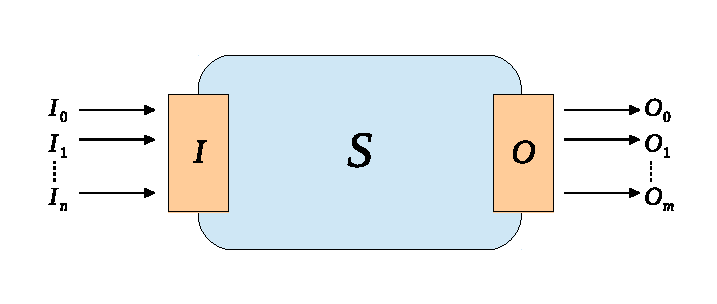
\includegraphics[width=0.65\textwidth]{figs/ch3/ws.eps}
    \caption{Un service Web atomique.}
    \label{fig:ch3/ws}
\end{figure}
%%% Local Variables:
%%% mode: latex
%%% TeX-master: "../../main"
%%% End:


Dans notre approche proposée, nous supposons que chaque service est
décrit par un document \acrshort{owls} qui possède un seule processus
atomique, et que chaque paramètre est annoté par un concept de
l'ontologie du domaine.\medskip

\begin{mydef}[\textbf{Annuaire des services Web}]
  Un annuaire des services Web est un ensemble
  $\mathpzc{R} =\{\mathit{S_0}, \mathpzc{S_1}, \dots,\mathit{S_n}\}$
  des services Web disponibles, où chaque
  $\mathpzc{S} \in \mathpzc{R}$ est un service Web décrit par un
  document \acrshort{owls}.
\end{mydef}

Afin de trouver un service composite exécutable à partir d'un annuaire
de services Web, un utilisateur doit fournir une requête de
composition.\medskip

\begin{mydef}[\textbf{Requête}]
  Une requête $\mathpzc{Q}$ est un 2-tuple $\mathpzc{<I_Q, O_Q>}$.
  $\mathpzc{I_Q}$ désigne la liste des paramètres d'entrée disponibles
  (fournit par l'utilisateur ou par un autre service client), et
  $\mathpzc{O_Q}$ la listes des paramètres de sortie requis
  (objectif).
\end{mydef}

Afin de découvrir et sélectionner un service Web composite suite à une
requête de composition $\mathpzc{Q}$, les services référencés dans un
annuaire doivent être structurés dans un graphe orienté modélisant
toutes les relations de dépendance fonctionnelle possibles entre les
services disponibles deux à deux.\medskip

%!TEX root = ../../main.tex
\begin{figure}[h]
    \centering
    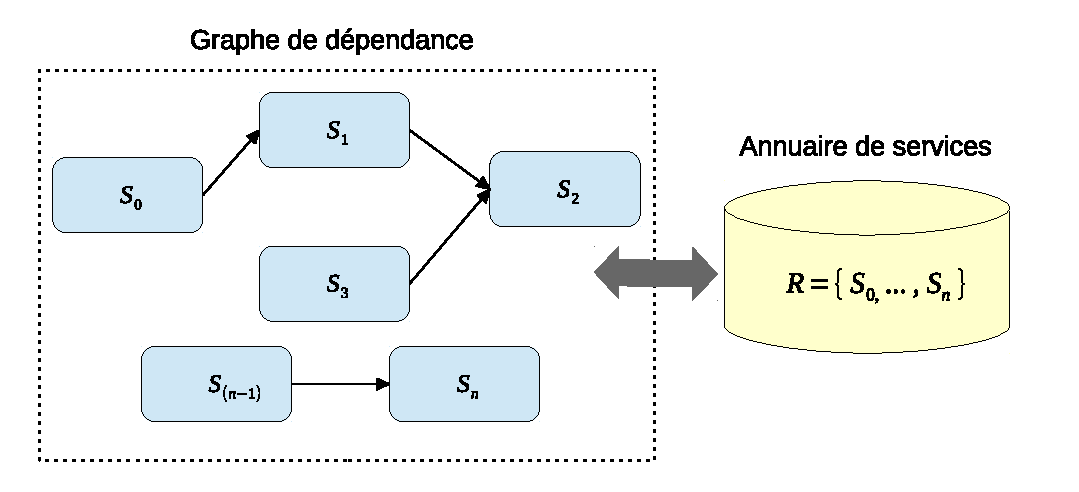
\includegraphics[width=1.1\textwidth]{figs/ch3/gd.eps}
    \caption{Graphe de dépendance $\mathpzc{GD}$ entre les services
      Web d'un annuaire $\mathpzc{R}$.}
    \label{fig:ch4/gd}
\end{figure}
%%% Local Variables:
%%% mode: latex
%%% TeX-master: "../../main"
%%% End:


\begin{mydef}[\textbf{Graphe de dépendance}]
  Un graphe de dépendance $\mathpzc{DG}$ est un ``graphe acyclique
  orienté'' $\mathpzc{DG}=<\mathpzc{R}, \mathpzc{L}>$ qui modélise
  toutes les relations de dépendance fonctionnelle possibles entre les
  services Web disponibles dans un annuaire $\mathpzc{R}$. Il existe
  une relation
  $\mathit{L_{ij}}=(\mathit{S_i}, \mathit{S_j}) \in \mathpzc{L}$ si et
  seulement s'il existe une relation de dépendance fonctionnelle entre
  $\mathit{S_i}$ et $\mathit{S_j}$, où
  $\{\mathit{S_i, S_j}\} \subset \mathpzc{R}$.\medskip
\end{mydef}

L'approche proposée consiste à construire un graphe de dépendance à
priori (\textit{Offline}) et le sauvegarder dans une base de données
graphe (\textit{Neo4j}). Suite à une requête $\mathpzc{Q}$, un
sous-graphe $\mathpzc{G}$ est extrait, qui correspond à un plan de
composition exécutable $\mathpzc{P}$ d'un service Web composite
satisfaisant.\medskip

%!TEX root = ../../main.tex
\begin{figure}[h]
    \centering
    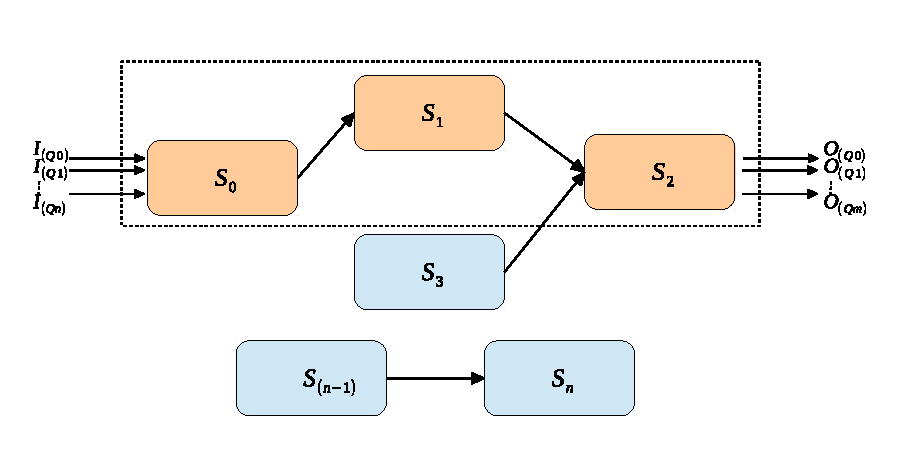
\includegraphics[width=1\textwidth]{figs/ch3/composition-plan.eps}
    \caption{Un service Web composite avec le plan de composition correspond.}
    \label{fig:ch3/composition-plan}
\end{figure}
%%% Local Variables:
%%% mode: latex
%%% TeX-master: "../../main"
%%% End:


\begin{mydef}[\textbf{Plan de composition}]
  Un plan de composition $\mathpzc{P}$ est un sous-graphe
  $\mathpzc{G \subset DG}$ d'un graphe de dépendance $\mathpzc{DG}$,
  tel que $\mathpzc{G=(R_Q,L_Q)}$ décrit le flux de données/contrôles
  d'exécution d'un ensemble de services Web atomiques
  $\mathpzc{R_Q \subset R}$ engagés dans un processus de
  composition. Il existe un lien de dépendance fonctionnelle
  (\textit{Link}) $\mathit{L_{Q_{ij}}} \in \mathpzc{L_Q}$ tel que
  $\mathit{L_{Q_{ij}}} = (S_i, S_j)$ si l'exécution d'un service
  $\mathit{S_j}$ dépend d'un ou plusieurs paramètres de sortie du
  $\mathit{S_i}$.\medskip
\end{mydef}

\begin{mydef}[\textbf{Service Web composite}]
  Un service Web composite $\mathpzc{S_Q}$ est un service Web
  exécutable composé de $n \geq 1$ services atomiques
  $\mathit{S_{0 \leq i \leq n}} \in \mathpzc{R_Q}$ tel que l'exécution
  d'un tel service correspond à l'exécution d'un plan de composition
  $\mathpzc{P}$ décrit par un graphe de dépendance
  $\mathpzc{G = <R_Q,L_Q>}$ suite à une requête $\mathpzc{Q}$.\medskip
\end{mydef}

La figure \ref{fig:ch3/composition-plan} montre un service Web
$\mathpzc{S_Q} = <\mathit{\{I_0, \dots, I_n\}}, \mathit{\{O_0, \dots,
  O_m\}}>$
correspondant à un plan de composition $\mathpzc{P}$ représenté par un
graphe de dépendances $\mathpzc{G =<R_Q,L_Q>}$, tel que
$\mathpzc{R_Q = \{S_0, S_1, S_2\}}$ et
$\mathpzc{L_Q = \{(S_0, S_1), (S_1, S_2)\}}$.\medskip

Une service Web composite $\mathpzc{S_Q = <I_S, O_S>}$ est créer et
exécuter suite à une requête de composition $\mathpzc{Q=<I_Q, O_Q>}$.
Deux conditions nécessaires et suffisantes pour que $\mathpzc{S_Q}$
satisfasse $\mathpzc{Q}$:\medskip

\begin{enumerateRoman}
\item L'interface d'entrée $\mathpzc{I_S}$ est équivalent, ou inclus
  dans $\mathpzc{I_Q}$ ($\mathpzc{I_S \subseteq I_Q}$).

\item L'interface de sortie $\mathpzc{O_Q}$ est équivalent, ou inclus
  par $\mathpzc{O_S}$ ($\mathpzc{O_Q \subseteq O_S}$).\medskip
\end{enumerateRoman}
\enddescription

Cette relation d'\emph{équivalence/inclusion} fonctionnelle entre les
interfaces d'\emph{entrée/sortie} sera abordée en détaille dans la
sections~\ref{sec:ch3/semantic-matching}.\medskip

\begin{mydef}[\textbf{Problème de composition}]
  Étant donné $\mathpzc{R}$ un annuaire des services Web et
  $\mathpzc{Q}$ une requête, Le problème de composition
  $\mathpzc{WCP=<R,Q>}$ consiste à trouver un plan optimal et
  exécutable de composition $\mathpzc{P}$ associé au service Web
  composite $\mathpzc{S_Q}$ satisfaisant la requête
  $\mathpzc{Q}$.\medskip
\end{mydef}

%!TEX root = ../../main.tex
\begin{figure}[h]
    \centering
    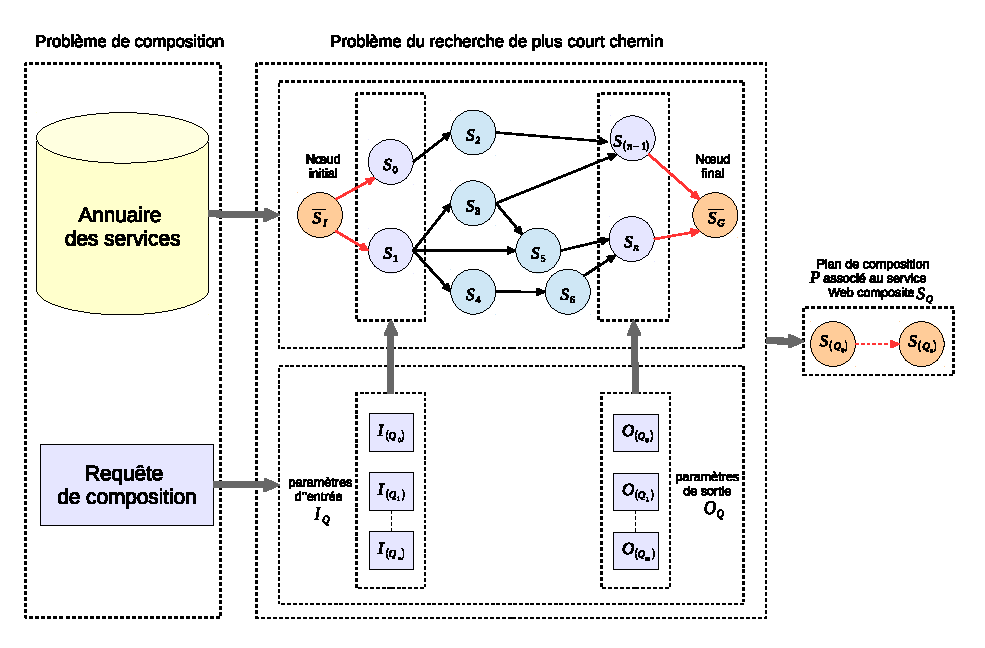
\includegraphics[width=1.15\textwidth]{figs/ch3/reformulation.eps}
    \caption{Reformulation du problème.}
    \label{fig:ch3/reformulation}
\end{figure}
%%% Local Variables:
%%% mode: latex
%%% TeX-master: "../../main"
%%% End:


La solution proposée dans ce chapitre s'appuie sur une transformation
du problème de composition défini précédemment
$\mathpzc{WCS \equiv <R,Q>}$ vers un problème du \textit{``plus court
  chemin dans un graphe orienté''}. Étant donné un graphe acyclique et
orienté $\mathpzc{DG}$, on souhaite de trouver le plus court chemin
entre un ensemble de nœuds initiales $\mathpzc{\overline{S_I}}$
(\emph{Initial services}) qui représentent l'ensemble de services du
départ, et l'ensemble de nœuds terminaux (\emph{Goal services})
$\mathpzc{\overline{S_G}}$ qui représentent les services d'arrivée,
tel que $\mathpzc{I_S \subseteq Inputs(\overline{S_I}) \subseteq I_Q}$
et
$\mathpzc{O_Q \subseteq Outputs(\overline{S_G}) \subseteq
  O_S}$.\medskip

La solution du notre problème sera donc le sous-graphe $\mathpzc{G}$
qui correspond à un plan de composition $\mathpzc{P}$. L'existence
d'une solution $\mathpzc{G}$ implique l'existence d'un service Web
composite $\mathpzc{S_Q= <R_Q, L_Q>}$, tel que
$\mathpzc{R_Q= <S_{Q_1}, \dots, S_{Q_n}>}$ et
$\mathpzc{\exists (S_{Q_i},S_{Q_g}) \in R_Q^2 \colon (S_{Q_i},S_{Q_g})
  \in (\overline{S_I} \times \overline{S_G})}$.\medskip

La figure~\ref{fig:ch3/reformulation} illustre graphiquement le
processus du reformulation. Les techniques et les algorithmes du
construction des graphes $\mathpzc{DG}$ et $\mathpzc{G}$, ainsi que
leurs structures et caractéristiques, seront présentés dans les
sections~\ref{sec:ch3/dependency-graph}
et~\ref{sec:ch3/composite-discovery}.\medskip

\section{Présentation de la solution proposée}
\label{sec:ch3/presentation}

\subsection{Objectifs et fonctionnalités principales}
\label{sec:ch3/presentation-goals}

L'objectif principal du système est la composition dynamique de
services web sémantiques disponibles dans un annuaire, en préservant
\emph{au préalable} toutes les dépendances fonctionnelles qui existent
entre eux dans une base de données graphe \emph{Neo4j} (approche
\emph{Offline}). En effet, notre système va profiter de l'un des
\acrshort{SGBD} graphe les plus évoluées et robustes aujourd'hui, ses
principales caractéristiques sont: la haute disponibilité, un système
transactionnel \acrshort{acid}, un langage de requête graphe
déclaratif, simple et efficace (\emph{Cypher}).\medskip

Le système assurera les fonctionnalités suivantes: la composition des
services, la découverte, l'exécution et la publication du service
composite.

\subsubsection{Acteurs intervenants}
\label{sec:ch3/presentation-actors}

\subsubsection{Diagramme de cas d’utilisation}
\label{sec:ch3/presentation-use-cases}

\newpage
\subsection{Architecture globale du système}
\label{sec:ch3/presentation-architecture}

% Description des Fonctionnalités du Système
L'architecture générale proposée pour la conception et la mise en
œuvre du notre système est illustrée dans la
figure~\ref{fig:ch3/architecture}.

 %!TEX root = ../../main.tex
\begin{figure}[h]
    \centering
    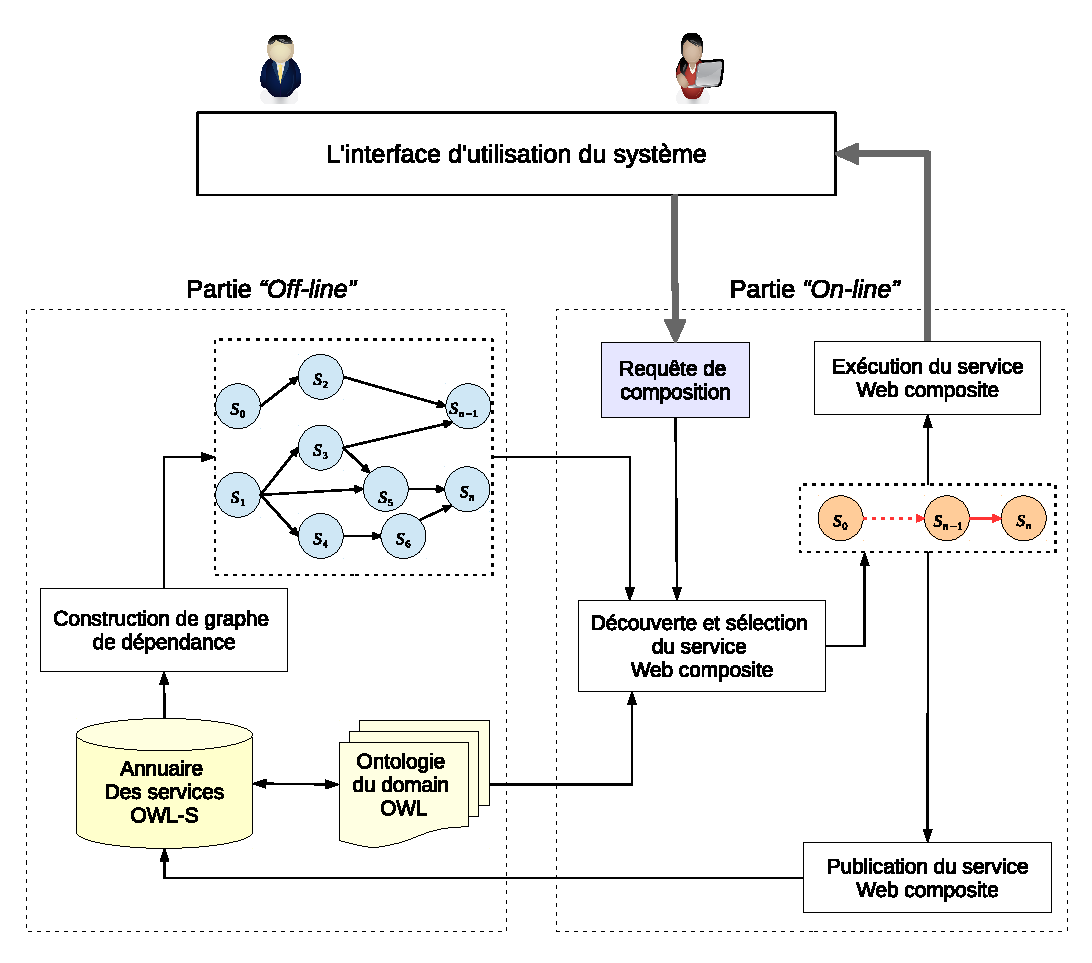
\includegraphics[width=1.15\textwidth]{figs/ch3/architecture.eps}
    \caption{Architecture générale du système.}
    \label{fig:ch3/architecture}
\end{figure}
%%% Local Variables:
%%% mode: latex
%%% TeX-master: "../../main"
%%% End:


\newpage
\section{Matchmaking sémantique de services Web}
\label{sec:ch3/semantic-matching}

% Définition: Lien sémantique (ou dépendance fonctionnelle)%
% Définition: Matching Quality of a Link

\section{Construction du graphe de dépendance}
\label{sec:ch3/dependency-graph}

\section{Découverte de services Web composites}
\label{sec:ch3/composite-discovery}

\section*{Conclusion}
\label{sec:ch3/conclusion}
\addcontentsline{toc}{section}{Conclusion} \markboth{CONCLUSION}{}


%%% Local Variables:
%%% mode: latex
%%% TeX-master: "../main"
%%% End:

\chapter{Une méthode de composition dynamique des services Web
  sémantiques utilisant Neo4j}
\label{ch:approche}

\section*{Introduction}
\addcontentsline{toc}{section}{Introduction} \markboth{INTRODUCTION}{}

\newpage
\section{Définitions préliminaires}
\label{sec:basic-defs}
Cette section a comme but d'introduire les notions de base ainsi que
les notations et terminologies \ref{sec:basic:ws} employées dans la
suite de ce chapitre. Nous présentons une formulation
mathématique de notre problème principal, à savoir \textit{la
  composition des servies Web} sous forme d'un problème de recherche
du plus court chemin dans un graphe orienté
\ref{sec:basic:composition}.\medskip

  \subsection{Services Web}
  \label{sec:basic:ws}
  Chaque service web peut contenir les définitions de différentes
  opérations identifiables par leurs noms et leurs paramètres. 
  Pour des raisons de simplicité, nous supposons que chaque service Web
  représente une seule opération.

  \begin{mydef}[\textbf{Service Web}]
    Un Service Web $S$ est un tuple $S = <I,O>$. $I/O$ qui désigne la
    liste des paramètres ``entrées/sorties'' où chaque paramètre est
    lié à un concept dans l'ontologie du domaine.
   \end{mydef}

  \input{figs/ch4/web-service.tex}

  Nous pouvons donc déterminer un service comme une application $S$
  définie par:

   \[ S =
     \begin{cases}
       Inputs^n  \to Outputs^m \\
       (i_0, ..., i_n ) \mapsto (o_0, ..., o_m)\\
     \end{cases}
   \]\medskip

   $S$ possède $n$ paramètres d'entrée notés $i_0...i_n$ et $m$
   paramètres de sortie notés $o_0,...o_m$. Dans notre approche
   proposée, nous supposons que chaque service est décrit par un
   document \textit{OWL-S} où chaque paramètre (d'entrée ou de sortie)
   est lié à un concept dans une ontologie \textit{(OWL)} du domaine
   local.\medskip


   Les ontologies de domaine locale sont les éléments essentiels des
   services web sémantique, et sont créées par les prestataires des services.
   Un fournisseur a besoin de cette classe lorsqu'il crée un service web
   sémantique ainsi que leur ontologie de description (\textit{OWL-S})
   pour pointer les paramètres de ce service vers des entités de cette
   classe.

   \begin{mydef}[\textbf{Annuaire des services Web}]
     un annuaire des services $R$ (ou référentiel des services) est un
     ensemble $R =\{s_0, s_1, ...s_n\}$ des services Web disponibles
     qui peuvent être composés suite à une requête du client de
     composition.
  \end{mydef}

  Dans notre architecture proposée, l'annuaire des services consiste
  en un service Web remplaçant un serveur \acrshort{uddi}. Ce service
  fournit l'ensemble des descriptions \textit{OWL-S} des services
  disponibles. Chaque document référence un document \acrshort{wsdl}
  qui à son tour pointe vers l'\acrshort{url} du service décrit
  (\textit{Endpoint}), les descriptions sémantiques des services Web
  disponibles seront stockées dans une base de données relationnelle
  et exposées via un simple interface \acrshort{rest}.\medskip

  %!TEX root = ../../main.tex
\begin{figure}[h]
    \centering
    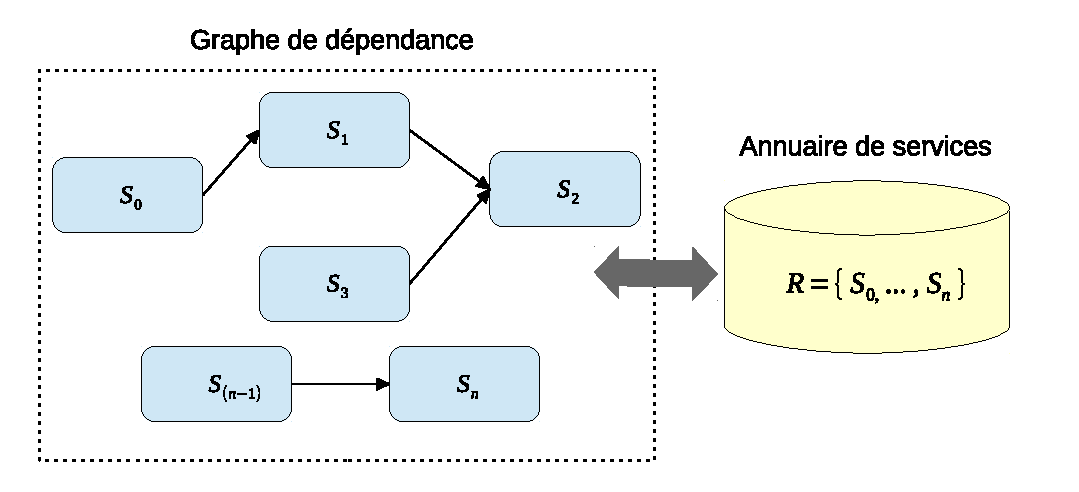
\includegraphics[width=1.1\textwidth]{figs/ch3/gd.eps}
    \caption{Graphe de dépendance $\mathpzc{GD}$ entre les services
      Web d'un annuaire $\mathpzc{R}$.}
    \label{fig:ch4/gd}
\end{figure}
%%% Local Variables:
%%% mode: latex
%%% TeX-master: "../../main"
%%% End:


  \subsection{Composition de services Web}
  \label{sec:basic:composition}
  Afin de découvrir et sélectionner un service Web composite suite à
  une requête du client de composition, les services référencés dans un
  annuaire doivent être structurés dans un graphe orienté modélisant
  toutes les relations de dépendance fonctionnelle possibles pour permettre 
  de réaliser un \textit{Matching} horizontal \ref{sec:ch4/matching}
  (la figure \ref{fig:ch4/gd}) entre les services disponibles deux à deux.\medskip

  \begin{mydef}[\textbf{Graphe de dépendance}]
    Un graphe de dépendance $GD$ est un ``graphe orienté et
    acyclique'' $GD=<R, E_r>$ qui modélise toutes les relations de
    dépendance fonctionnelle possibles entre les services Web
    disponibles dans un annuaire $R$. Il existe une relation $e=(s_0,
    s_1) \in E_r$ si et seulement si il existe une relation de
    dépendance entre $s_0$ et $s_1$.
  \end{mydef}

  L'approche proposée consiste à construire le graphe de dépendance à
  priori (\textit{Offline}) et le sauvegarder dans une base de données
  graphe (\textit{Neo4j}). Suite à une requête $Q$, un sous-graphe $G$
  est extrait reflétant un plan de composition exécutable $P$ d'un
  service Web composite satisfaisant.

  \begin{mydef}[\textbf{Requête}]
    Une requête $Q$ est un tuple $Q = <I', O'>$. $I'$ désigne la liste
    des paramètres d'entrée fournis par le client et $O'$ représente
    la listes des paramètres requis (sorties).
  \end{mydef}

  %!TEX root = ../../main.tex
\begin{figure}[h]
    \centering
    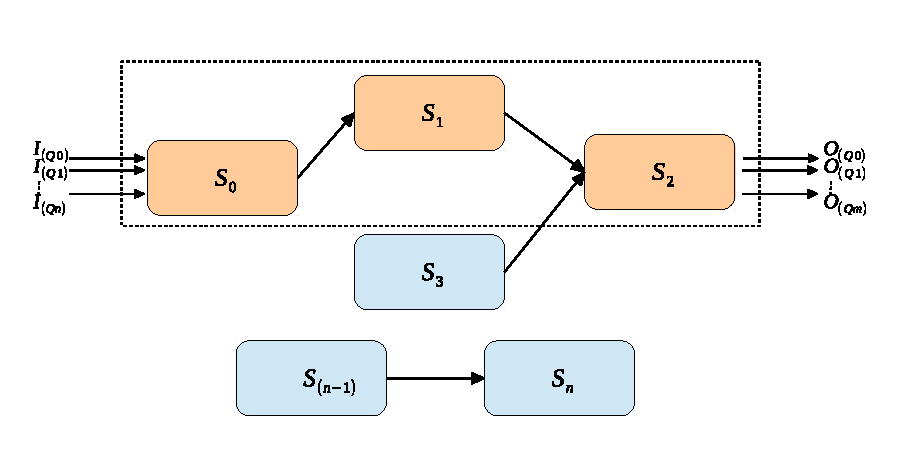
\includegraphics[width=1\textwidth]{figs/ch3/composition-plan.eps}
    \caption{Un service Web composite avec le plan de composition correspond.}
    \label{fig:ch3/composition-plan}
\end{figure}
%%% Local Variables:
%%% mode: latex
%%% TeX-master: "../../main"
%%% End:


  \begin{mydef}[\textbf{Plan de composition}]
    Un plan de composition $P$ est un sous-graphe
    $G$``\textbf{connexe''} d'un graphe de dépendance $GD$, $G=(V,E)$
    tel que $G \subset GD$ décrit le flux de données/contrôles
    d'exécution d'un ensemble de services Web atomiques $V \subset R$
    engagés dans un processus de composition. Il existe une arête $e
    \in E$ tel que $e = (s_i, s_j)$ si l'exécution d'un service $s_j$
    dépend d'un ou plusieurs paramètres de sortie de $s_i$.
  \end{mydef}

  \begin{mydef}[\textbf{Service Web composite}]
    Un service Web composite $S_c$ est un service Web exécutable
    composé de ``$n$'' services atomiques $s \in \{s_0,..., s_n\}$ tel
    que $n \succeq 1$, l'exécution d'un service Web composite
    correspond à l'exécution d'un plan de composition $P$ décrit par
    $G=<V,E>$ où $V = \{s_0, ..., s_n\}$ et $E$ décrivent les
    relations de dépendance entre les services $V$.
  \end{mydef}

  La figure \ref{fig:ch4/composition-plan} montre un service Web
  composite $S_c = <\{i_0, i_1\}, \{o_0, o_1\}>$ correspondant à un
  plan de composition $P$ représenté par un graphe\\ $G =<\{s_0, s_1,
  s_2, s_4\}, \{(s_0, s_1), (s_1, s_2), (s_2, s_4)\}>$.

\section{Architecture proposée}
\label{sec:proposition}

\section{Matching des services  atomiques}
\label{sec:ch4/matching}

\section{Construction et persistance du graphe de dépendance dans une
  base de données Neo4J}
\section{Découverte et exécution des services composites}

\section*{Conclusion}
\label{sec:conclusion}
\addcontentsline{toc}{section}{Conclusion} \markboth{CONCLUSION}{}


%%% Local Variables:
%%% mode: latex
%%% TeX-master: "../main"
%%% End:


\bibliographystyle{unsrt-fr}
\bibliography{references}
\addcontentsline{toc}{chapter}{bibliographie}

\begin{appendices}
% !TEX root = ../main.tex
\chapter{Le Web sémantique}
\label{annexe:semantic-web}
% TOOD: les ordinateurs et les utilisateurs VS
% ordinateurs et utilisateurs.

% the original text:
% ``The Semantic Web is an extension of the
% current web in which infor- mation is given well-defined meaning,
% better enabling computers and people to work in cooperation.''

L'expression \emph{``Web sémantique''} trouve ces origines dans un
article original publié par Tim Berners-Lee \emph{et
  al.}~\cite{berners2001semantic} en \date{2001}. Le terme fait d'abord
référence à la vision du Web de demain comme un vaste espace d'échange
de ressources entre les êtres humains et les machines permettant une
exploitation, qualitativement supérieure, de grands volumes
d'informations et de services variés. D'après ses fondateurs
\emph{``le Web sémantique est une extension du Web actuel avec une
  signification bien définie des informations. Il permet une meilleur
  coopération et d'échanger l'information entre les ordinateurs et les
  utilisateurs.''}\medskip



\newpage
\section{La vision du Web sémantique}
\label{sec:semantic-web-vision}

Le Web actuel est essentiellement \emph{\textbf{syntaxique}}, dans le
sens que la structure des documents est bien définie mais que son
contenu reste quasi inaccessible aux traitements machines. Il s'agit
d'un Web de documents, les resources sont structurées en
\acrshort{html}, identifiés de manière unique par des \acrshort{uri}
reliés entre eux par des liens hypertextes. L'information est
essentiellement textuelle et la strucure riche qui est généralement
conçus au préalable dans des schémas relationnelles est presque
complètement perdu dans le processus de publication de telles données
sous formes des documents \acrshort{html}. La nouvelle génération de
Web nommée \emph{``Le Web sémantique''} a pour ambition de lever cette
difficulté. Les ressources du Web seront plus aisément accessibles
aussi bien par l'homme que par la machine, grâce à la représentation
\emph{\textbf{sémantique}} de leurs contenus.\medskip

\section{La description des ressources Web: RDF}
\label{sec:semantic-web-rdf}
%% Dans cette section on va parler de RDF/RDFS

\section{Langage de définition des ontologies: OWL}
\label{sec:semantic-web-owl}

% What is semantic web?

% Le Web tel que nous le connaissons aujourd'hui est encore conforme à
% la vision initiale.

% Le Web a été conçu principalement pour une utilisation par les
% humains. Néanmoins, il existe un effort visant à automatiser son
% utilisation et d'être plus accessible pour les machines.

% \cite{bartalos2011effective} The Web was primarily designed for use
% by humans. Nevertheless, there is an effort to automate its use and
% bring the Web more accessible for machines. This has brought forward
% the need for machine processable representations of semantically
% rich information. This has brought forward the need for machine
% processable representations of semantically rich information: a
% vision at the heart of the Semantic Web

% Dans un premier temps, on va essayer de clarifier la notion d'un
% service Web sémantique, puis étudier les langages émergeants qui
% permettent de décrire ce type de service Web.

% L'objectif premier du Web sémantique est de définir et lier les
% ressources du Web afin de simplifier leur utilisation, leur
% découverte, leur intégration et leur réutilisation dans le plus
% grand nombre d'applications \cite{berners2001semantic}. Le Web
% sémantique doit fournir l'accès à ces ressources par l'intermédiaire
% de descriptions sémantiques exploitables et compréhensibles par des
% machines. En effet, Les technologies du Web sémantique complètent le
% Web actuel avec des outils sémantiques. Il ne s'agit donc pas de
% créer un nouveau Web ou un Web séparé de l'existant : ce Web de
% données repose entièrement sur les technologies et concepts qui ont
% fait le succès du Web tel que nous le connaissons aujourd'hui
% \cite{bertails2010web}.

% La réalisation du Web sémantique trouve ces racines dans le
% développement des langages de balises inspiré par des travaux issus
% de la communauté AI \cite{mcilraith2001semantic}, tels que
% \textsc{OIL} \cite{fensel2001oil}, \textsc{DAML+OIL}
% \cite{horrocks2002daml+oil} et \textsc{DAML+OTN}
% \cite{mcguinness2003daml} (ces deux derniers langages font partie de
% la famille \acrshort{daml}).

% TODO refactor Ces langages ont une sémantique bien définies et
% permettent le balisage et la manipulation des taxonomies complexe et
% des relations logiques entre les entités sur le
% Web. \cite{fensel2000creating}

% \input{figs/3w_to_sws.tex}

% Cette description repose sur des ontologies. Selon Gruber
% \cite{gruber1993translation}, une ontologie est une spécification
% explicite d'une conceptualisation. Une conceptualisation est un
% modèle abstrait qui représente la manière dont les personnes
% conçoivent les choses réelles dans le monde et une spécification
% explicite signifie que les concepts et les relations d'un modèle
% abstrait reçoivent des noms et des définitions explicites. Le Web
% sémantique est devenu un domaine à part entière, preuve en est la
% création en 2001 du groupe de travail sur ce sujet par le
% \textsc{W3C}.

%%% Local Variables:
%%% mode: latex
%%% TeX-master: "../main"
%%% End:

\chapter{Vers les bases de données graphe}
\label{annexe:graph-db}

Avec le développement rapide et continu de l'\textit{Internet} et du
\textit{cloud computing}, divers types d'applications ont émergés, ce
qui augmente l'importance accrue de la technologie de base de données,
notamment dans les aspects suivants \cite{han2011survey}:

\begin{itemize}\renewcommand\labelitemi{--}
\item Haute concurrence de lecture et d'écriture avec une faible
  latence.

\item Stockage et la gestion d'une grande masse de données \emph{(Big
    Data)}.

\item Haute scalabilité (évolutivité) et disponibilité.\medskip
\end{itemize}
\enddescription

Bien que les bases de données relationnelles ont occupé une grande
position dans le domaine de stockage de données, le modèle relationnel
commence à montrer ses limites en faisant face aux plusieurs
exigences: \cite{han2011survey}: lente lecture et l'écriture, capacité
limitée, difficulté d'expansion et scalabilité, etc. Afin de faire
face aux limitations ci-dessus, une variété de nouveaux types de bases
de données ont apparus qui s'affranchissent du modèle relationnel
pour miser sur le partitionnement horizontal et le relâchement des
contraintes d'intégrité, ce modèle émergent est appelé le modèle
\acrshort{nosql}.\medskip

Dans ce chapitre, nous exposons les différentes approches et
plateformes du stockage \acrshort{nosql} les plus connues dans
l'industrie tout en mettant l'accent sur les bases de données graphe
(et \emph{Neo4j} particulièrement). Nous commençons d'abord par
présenter les quatre catégories majeures des systèmes
\acrshort{nosql}. Ensuite, nous nous focalisons sur les \acrshort{SGBD}
orientés graphes, leurs différents modèles et implémentations ainsi
que les langages de requêtes les plus adoptés pour les interroger.

\section{L'environnement NoSQL}
\label{sec:nosql}
\acrshort{nosql} désigne une nouvelle génération de technologies de
gestion des bases de données conçu pour répondre à l'augmentation du
volume des données stockées, traitées et analysées par les entreprises
et organisations ayant une large étendue d'utilisateurs tels que
Google, Amazon, Facebook et Twitter, \acrshort{nosql} comprend une
multitude de systèmes de gestion de données qui ne sont plus fondés
sur l'architecture classique des bases relationnelles. L'unité logique
n'y est plus la table, et les données ne sont en général pas
manipulées avec \textsc{SQL}.  D'après Fowler \textit{et al.}
\cite{sadalage2012nosql}, Les caractéristiques communes des bases de
données \acrshort{nosql} sont:

\begin{itemize}\renewcommand\labelitemi{--}
\item Ne sont pas fondées sur de le modèle relationnel classique.
\item Optimisées pour les environnements distribués.
\item Construites pour les applications Web modernes avec une grande
  masse de données.
\item \emph{Schemaless} (il n'existe plus d'intégrité référentielle ou
  schéma prédéfini).
\end{itemize}

  \subsection{Les catégories des bases de données NoSQL}
  \label{sec:cat-nosql}
  Il existe dans la mouvance \acrshort{nosql} une diversité importante
  d'approches que nous classons en quatre grandes catégories
  \cite{sadalage2012nosql}: dépôts \textit {clés/valeurs}, bases
  orientées documents, orientées colonnes, et bases orientées
  graphe.\bigskip

  \textsf{Dépôts clés/valeurs}: Le principe des bases
  \textit{clé/valeur} est de stocker les données sous une forme
  simple: une \emph{clé } (chaîne de caractères) associée à une
  \emph{valeur} d'une forme libre (chaîne de caractère, ou bien un
  objet sérialisé), cette clé est utilisée pour toutes les opérations
  à effectuer sur les données telles que l'insertion, la mise à jour
  et la suppression. Bien que la structure est plus simple, la vitesse
  d'interrogation est extrêmement supérieur à la base de données
  relationnelles favorisant la scalabilité (\emph{scalability}) plus
  que la cohérence, on les retrouve très souvent comme système de
  stockage de cache ou de sessions distribuées, notamment là où
  l'intégrité relationnelle des données est non significative. Les
  solutions les plus connues, telles que \emph{Redis}, \emph{Riak} et
  \emph{Voldemort} sont principalement influencées par le projet
  \emph{Dynamo} d'Amazon \cite{decandia2007dynamo}.\bigskip

  \textsf{Orientées documents}: Cette famille de base de données est
  une évolution de la base de données \textit{clé/valeur} destinée aux
  applications qui gèrent des documents (généralement du format
  \textsc{JSON} ou \textsc{XML}) où chaque clé n'est plus associée à
  une valeur sous forme de bloc binaire mais à un document dont la
  structure reste libre (\textit{scheme-less}). L'avantage est de
  pouvoir récupérer, via une seule clé, un ensemble d’informations
  structurées de manière hiérarchique, ainsi le stockage de
  volumes très importants de données pour lesquelles la modélisation
  relationnelle aurait entraînée une limitation des possibilités de
  partitionnement et de réplication. Les deux implémentations les plus
  populaires dans cette catégorie sont \emph{CouchDB} d'Apache et
  \emph{MongoDB}.\bigskip

  \textsf{Orientées colonnes}: La famille des stockages orientés
  colonnes sont une évolution du modèle \textit{clé/valeur} utilisant
  des \textit{``familles''} afin de grouper certaines lignes. Ces
  familles peuvent devenir hiérarchiques et les relations entre les
  données deviennent explicites. Une base de données orientées
  colonnes permet de plus une compression par colonne, efficace
  lorsque les données de la colonne se ressemblent. Comme solutions,
  on retrouve principalement \emph{HBase}, \emph{HyperTable}
  (implémentations Open Source du modèle \emph{BigTable}
  \cite{chang2008bigtable} publié par Google) ainsi que
  \emph{Cassandra} (projet Apache qui respecte l'architecture
  distribuée de \emph{Dynamo} \cite{decandia2007dynamo} d'Amazon et le
  modèle BigTable de Google).\bigskip

  \textsf{Orientées graphes}: Ce paradigme est le moins connu de ceux
  de la mouvance \acrshort{nosql}. Ce modèle s'appuie principalement
  sur deux concepts: d'une part l'utilisation d'un moteur de stockage
  pour les objets (qui se présentent sous la forme d'une base
  documentaire, chaque entité de cette base étant nommée
  \emph{nœud}). D'autre part, à ce modèle, vient s'ajouter un
  mécanisme permettant de décrire les relations entre les objets
  (\emph{arcs}). Principalement, ces bases de données sont nettement
  plus efficaces que leur précedente relationnelle pour traiter les
  problématiques liées aux réseaux.  En effet, lorsqu'on utilise le
  modèle relationnel, cela nécessite un grand nombre d'opérations
  complexes (souvent, des jointures trop lentes) pour obtenir des
  résultats. Dans cette catégorie on peut citer \emph{Neo4j},
  \emph{OrientDB}, \emph{Titan} et \emph{AllegroGraph} comme les
  implémentations les plus répondues de ce modèle.

  \subsection{Le théorème de CAP }
  \label{sec:cap}
  \acrshort{cap} \cite{brewer2000towards} est l'acronyme de
  \textit{``\textbf{C}onsistency, \textbf{A}vailability and
    \textbf{P}artition Tolerance''}, ou \textit{``Cohérence,
    Disponibilité et Résistance au partitionnement''}. Ce théorème
  explique qu'il est impossible qu'un système distribué satisfasse
  simultanément aux trois contraintes suivantes:\medskip

  \renewcommand{\descriptionlabel}[1]{\hspace{1cm}\textbullet~\textsf{#1}}
  \begin{description}
  \item [Cohérence]: tous les nœuds du système voient exactement les
    mêmes données au même moment.

  \item [Disponibilité]: la perte de nœuds n'empêche pas les
    survivants de continuer à fonctionner correctement.

  \item [Résistance au partitionnement]: aucune panne moins importante
    qu'une coupure totale du réseau ne doit empêcher le système de
    répondre correctement.
  \end{description}
  \enddescription
  \bigskip

  \input{figs/cap.tex}

  \newpage

  Les bases de données relationnelles implémentent les propriétés de
  cohérence et de disponibilité (système \emph{CA}). Les bases de
  données \emph{NoSQL} sont généralement des systèmes \emph{CP}
  (cohérent et résistant au partitionnement) ou \emph{AP} (disponible
  et résistant au partitionnement), la figure \ref{fig:cap} montre
  le positionnement de quelque systèmes \emph{NoSQL} par rapport au
  théorème \acrshort{cap}.

\section{Bases de données orientées graphes}
\label{sec:graph-database-overview}
En raison du volume exponentiellement croissant de données ouvertes
disponibles, l'intérêt pour les systèmes de gestion de bases de
données graphe est grandissant. Ces systèmes permettent de manipuler
des données structurées sous forme de graphe, auxquelles aucun schéma
n'est a priori associé. Ainsi, les systèmes de gestion de bases de
données graphe permettent entre autres la gestion de données des
réseaux sociaux, de données \textit{bio-informatiques}, et de données
issues du Web sémantique tels que des documents \acrshort{rdf}
éventuellement issus de l'exploitation des données ouvertes. De
nombreux systèmes permettant la gestion des bases de données graphe
sont apparus. Il s'agit par exemple de \textit{AllegroGraph}
\textit{InfiniteGraph}, \textit{Neo4j} ou \textit{Sparksee}.\medskip

Cette section a pour but d'introduire les modèles de données utilisés
pour la persistance des données hautement connectées
\ref{sec:persistence}, ainsi que les techniques du stockage
sous-jacent et d'indexation utilisées par les différents systèmes de
gestion des bases de données graphe.
\ref{sec:graph-internals}.\medskip

  \subsection{Définitions et caractéristiques}
  \label{sec:graphdb-defs}
  % Les bases de données orientées graphes sont conçues pour modéliser
  % des réseaux de données fortement connectées et y naviguer facilement
  % en bénéficiant de performances extrêmement élevées.\medskip

  Selon Robinson \emph{el al.} \cite{robinson2013graph} \textit{``Un
    système de gestion de base de données orienté graphe (ou
    simplement, une base de données graphe) est un système de gestion
    de base de données en ligne avec les quatre
    opérations de base pour la persistance des données
    (\acrshort{crud}) exposant une structure de donnée
    graphe.''}\bigskip

  Angles et Gutierrez \cite{angles2008survey} conceptualise les
  bases de données graphe (\textit{``graph db-model''}) en trois
  éléments fondamentaux:\medskip
  \newpage
  \renewcommand{\descriptionlabel}[1]{\hspace{1cm}\textbullet~\textsf{#1}}
  \begin{description}
  \item [Modèle de données]: une base de donnée graphe permet la
    modélisation, le stockage et la manipulation des données complexes
    liées par des relations non-triviales ou variables. Elle stocke
    les données en graphe ou en une structure de données plus générique
    (\textit{hypergraphs} ou \textit{hypernodes}) capable de
    représenter avec élégance n'importe quel type de données d'une
    manière ultra accessible. Un graphe contient des \textit{nœuds} ,
    reliés par des \textit{relations}. Dans le modèle de graphe à
    propriétés, chaque nœud et relation peut être libellée et contenir
    plusieurs \textit{propriétés} les décrivant. Les relations entre
    les nœuds sont un élément clé d'une base de données graphe, elles
    permettent de trouvent les données reliées, tout comme les
    noeuds.\medskip

  \item [Manipulation de données]: Les manipulations de données sont
    exprimées par des transformations de graphe ou des
    \textit{traversées}, ces opérations utilisent les primitives
    fondamentales d'une structure de données graphe, comme les
    relations d'adjacence entre les nœuds, les chemins de parcours,
    les sous-graphes et  la notion de connectivité, etc. Ces opérations
    sont utilisées pour la création, l'interrogation et la mise à jour
    d'une base de données graphe. Une \textit{traversée} consiste à
    la manière dont les données sont interrogées dans un graphe,
    naviguant depuis les nœuds de départ vers les noeuds reliés en
    accordance avec un algorithme.\medskip

  \item [Les contraintes d'intégrité]: une contrainte d'intégrité
    permet de garantir la cohérence des données lors des mises à jour,
    ces contraintes nous permettent, par exemple, de typer des nœuds,
    définir des contraintes d'unicité sur certains champs, etc.
  \end{description}
\enddescription

  \subsection{Techniques de persistance des bases de données graphes}
  \label{sec:persistence}
  Généralement, nous pouvons distinguer trois techniques majeures de
  stockage adoptés par les systèmes de gestion des bases de données
  graphe: les bases de données graphe qui utilisent des
  \acrshort{SGBDR} comme un \emph{backend}, celles qui utilisent des
  systèmes \acrshort{nosql}, et enfin, nous avons les bases de données
  graphe natives qui fournissent ses propres implémentations de
  stockage.

    \subsubsection{Bases de données graphe au-dessus d'un stockage
      SQL}
    \label{sec:graphdb-over-sql}
    Une base de donnée graphe peut être stockée dans une base de
    données relationnelle. Les étiquettes et les attributs de nœuds et
    arcs peuvent être gérés séparément dans d'autres tables et renvoyés
    par des clés étrangères. l'utilisation des \acrshort{SGBDR} comme
    un moteur de stockage a quelques avantages : des systèmes
    d'indexation évolués, un support des transactions sophistiqué, et
    le langage de requêtes \emph{SQL} qui est un standard bien établi
    avec un cycle d'apprentissage rapide.\medskip

    \input{figs/periscope-gq.tex}

    Cette classe comprend \emph{GRIPP} \cite{trissl2007fast}, et
    Periscope/GQ \cite{tian2008periscope} qui implémente un système de
    gestion des bases de données graphe comme une application
    au-dessus d'un moteur de stockage relationnel \emph{PostgreSQL}.

    \newpage
    \subsubsection{Bases de données graphes au-dessus d'un stockage
      NoSQL}
    \label{sec:graphdb-over-nosql}
    Plusieurs systèmes de base de données graphe utilisent des
    systèmes \acrshort{nosql} comme un moteur de stockage interne
    offrant une meilleure scalabilité et un support fiable pour le
    partitionnement des données.\bigskip

    \textsf{HypergraphDB} \cite{hypergraphdb,
      iordanov2010hypergraphdb} est une base de donnée qui implémente
    le modèle de données \emph{``hypergraph''} où la notion d'un arc
    est étendue pour pouvoir connecter plus de deux nœuds, ce qui est
    particulièrement utile pour la modélisation des données telles que
    la représentation des connaissances, l'intelligence artificielle
    et la bio-informatique. \emph{HypergraphDB} utilise le modèle
    \textit{clé/valeur} de \emph{BerkeleyDB} \cite{berkeleydb} pour
    stocker toutes les informations relatives au graphe sous forme de
    pairs \textit{clé/valeur}, chaque objet du graphe (nœud ou arc)
    est identifié par une clé unique (appelée atome). Chaque atome est
    lié à un ensemble d'atomes par une relation de type \emph{0:N}
    (zéro ou plusieurs atomes), ces relations forment également la
    structure typologique ``hypergraph''.\bigskip

    \textsf{OrientDB} \cite{orientdb} est un système hybride de
    gestion de base de données graphes qui combine les fonctionnalités
    d'une base orientée document et une base orientée graphe avec
    une capacité de stockage des données structurées ou
    semi-structurées (\emph{schema-less}). il supporte aussi la
    répartition de charge à travers plusieurs machines et la
    réplication multi-maîtres tout en assurant les propriétés
    \acrshort{acid} des données. Pour les requêtes simples,
    \emph{OrientDB} s'appuie sur \emph{SQL} et utilise des langages de
    parcours des graphes comme \emph{Gremlin} afin d'éviter les
    jointures \emph{SQL} coûteuses pour les requêtes
    complexes.\bigskip

    \textsf{Titan} \cite{titan} est une base de données orientée
    graphe évolutive (\emph{scalable}) et transactionnelle. Elle est optimisée
    pour le stockage et l'interrogation des données graphes contenant
    des centaines de milliards de sommets et d'arcs à travers un
    \emph{cluster} multi-machine avec des schémas complexes du
    parcours et requêtage et une exécution en temps réel. \emph{Titan}
    utilise une multitude de systèmes \emph{NoSQL} comme un moteur de
    stockage (\emph{backend}), par exemple, \emph{Hbase},
    \emph{Cassandra}, \emph{BerkeleyDB}, cette diversité offre une
    flexibilité en terme des caractéristiques \emph{CAP} \ref{sec:cap}
    assurées par le système.

    \subsubsection{Les bases de données graphe natives}
    \label{sec:graphdb-native}
    Les bases de données graphe natives possèdent leur propre
    système de fichiers pour stocker les données au lieu de compter
    sur des moteurs de stockage tiers. Ces bases de données sont
    optimisées pour stocker et gérer les données \textbf{fortement}
    connectées où la performance et la disponibilité sont
    primordiales.\bigskip

    % TODO: enhance
    \textsf{Neo4j} \cite{neo4j} est un système de gestion de base de
    données graphe \textit{open-source} populaire implémenté en
    \textit{java} et supporté commercialement par \textit{Neo
      Technology}\footnote{\url{http://neo4j.com/}}. il a été
    conceptualisé et construit depuis le début afin d'être un système
    fiable, robuste, évolutif et très performant optimisé pour stocker
    et gérer des grandes masses de données structurées en graphe,
    \textit{Neo4j} convient aussi bien pour le déploiement en grande
    entreprise pour des projets plus légers en utilisant une
    partie du serveur. Parmi ses fonctionnalités:\medskip

    \begin{itemize}\renewcommand\labelitemi{--}
    \item Transactions \acrshort{acid} réelle avec une haute disponibilité.
    \item Supporte jusqu'à des milliards de noeuds et relations.
    \item Requêtes ultra-rapides grâce aux traversées.
    \end{itemize}
    \enddescription
    \medskip

    \textit{Neo4j} est fourni avec une \textit{API} basée sur des
    \textit{callbacks}, ce qui laisse la possibilité de spécifier
    les règles pour les traversées, Les autres options pour traverser
    ou interroger un graphe dans \textit{Neo4j} sont \textit{Gremlin}
    \ref{sec:gremlin} et \textit{Cypher} \ref{sec:cypher}.\bigskip

    \textsf{AllegroGraph} \cite{allegrograph} est un système performant
    de persistance des données graphes avec un stockage natif,
    implémenté initialement comme un système de persistance et
    gestion de documents \acrshort{rdf} doté d'une interface
    \acrshort{rest} \cite{fielding2000architectural}. Similaire à
    \emph{Neo4j}, \emph{Allegrograph} garantit la satisfaction des
    propriétés \acrshort{acid},  d'atomicité, cohérence, isolation et
    durabilité. \emph{AllegroGraph} supporte \acrshort{sparql}, RDFS++
    et \textit{Prolog} pour des applications clientes
    multiples.\bigskip

    \textsf{Sparsity} \cite{sparksee} (auparavant connu sous le nom
    \emph{DEX}) est un système natif de stockage de données graphe
    persistantes et temporaires. \emph{Sparsity} focalise sur la
    gestion et l'interrogation à haute performance des bases de 
    données graphes de grande taille. En encodant les matrices d'adjacences en
    \emph{bitmap}, le système a une gestion d'espace disque compacte et
    efficace et assure une très bonne performance.\medskip
    \newpage

    \textsf{InfiniteGraph} \cite{infinitegraph} est un système
    distribué de gestion des bases de données graphe qui supporte des
    grandes masses évolutives de données (\emph{large-scale}) avec une
    capacité d'analyse efficace des graphes et une bonne prise en
    charge des algorithmes distribués du
    parcours. \emph{InfiniteGraph} fournit une variété
    d'implémentations pour des différents systèmes (serveurs
    d'application, les plateformes de \emph{cloud computing} et les
    systèmes embarqués).

  \subsection{Techniques de stockage et d'indexation}
  \label{sec:graph-internals}
  Il ya plusieurs façons pour représenter un graphe dans une mémoire
  principale d'un système de stockage. On dit qu'un système de gestion
  des bases de données graphe dispose des capacités \emph{natives} de
  parcours des graphes s'il possède une propriété fondamentale
  appelée \emph{index-free adjacency}.

  \input{figs/gpi.tex}
  \newpage

    \subsubsection{Index-free adjacency}
    \label{sec:index-free}
    Dans un système de stockage de base de données graphe qui utilise
    la technique \emph{index-free adjacency}, chaque noeud maintient
    des références directes à ses noeuds adjacents agissant comme un
    micro index d'autres noeuds voisins. Cette méthode améliore la
    fiabilité du système de stockage d'une façon considérable
    comparant à celles qui utilisent un index global. En effet, le temps
    de réponse des requêtes est indépendant de la taille globale du
    graphe. Pour traverser un graphe d'une taille donnée $n$ à $m$
    pas, le coût est d'ordre $\mathcal{O}(m\log{}n)$ dans un système
    avec un index global, et d'ordre $\mathcal{O}(m)$ pour un système
    natif qui utilise un \emph{index-free adjacency}.

    \input{figs/vertex-centric-indices.tex}

    \subsubsection{Vertex Centric Indices}
    \label{sec:vertex}

    L'objectif de cette technique est de trier et indexer tous les arcs
    incidents d'un noeud (et donc les noeud adjacents) selon les
    propriétés de ces arcs. Ces indexes éliminent la nécessité de
    balayage linéaire des arcs incidents lors d'une requête de parcours
    ($\mathcal{O}(n)$) en faveur d'un parcours plus rapide
    ($\mathcal{O}(\log{}n)$). Cette méthode est utilisée par (\emph{Titan}
    \cite{vertexci}) surtout pour confronter le problème de
    \emph{Supernode} dans les graphes fortement connectés, un
    \emph{Supernode} est un noeud avec un très grand nombre d'arcs
    incidents.

  % \newpage
  % \subsection{Comparaison}
  % \label{sec:graphdb-comp}
  % \input{tables/graphdb-comp.tex}
  % \newpage

  % {\color{red}
  %   to be continued
  % }
  % \newpage

\section{Langages des requêtes}
\label{sec:query-languages}
Les langages des requêtes ont toujours été la clé du succès des
\acrshort{SGBD}. La prévalence des \emph{\acrshort{SGBDR}} dans les
dernières décennies est étroitement couplée avec le succès du
\emph{SQL}. Des divers langages ont été définis pour exprimer des
requêtes vis-à-vis plusieurs dépôts de données, par exemple,
\emph{XQuery} \cite{boag2002xquery} et \emph{XPath}
\cite{clark1999xml} pour les bases de données \emph{\acrshort{xml}},
\emph{QQL} \cite{alashqur1989oql} pour les bases de données orientées
objet et \acrshort{sparql} \cite{prud2008sparql} pour les
triplestores (les bases de données \emph{RDF}). Cette section présente
trois langages des requêtes largement supportés par les systèmes de
gestion des bases de données graphe.

% \input{figs/query-graph-example.tex}

% Le graphe présenté par la figure \ref{fig:query-graph-example} sera
% utilisé pour illustrer la syntaxe et la sémantique de ces trois
% langages. Le graphe représente le résultat d'un processus de
% \emph{matching} sémantique entre cinq services Web qui forment un plan de
% composition.

  \subsection{SPARQL}
  \label{sec:sparql}
  \acrshort{sparql} \cite{prud2008sparql} est un langage populaire de
  requête pour les données \acrshort{rdf}, il est reconnu comme l'une
  des technologies clés du Web sémantique. Le standard
  \acrshort{sparql} est largement utilisé pour exprimer des
  interrogations à travers diverses sources de données graphe comme
  des triplestores \acrshort{rdf}. Il est capable de rechercher des
  motifs de graphe (\emph{graph patterns}) ainsi que leurs
  conjonctions et leurs disjonctions. Les résultats des interrogations
  \acrshort{sparql} peuvent être des ensembles de résultats ou des
  graphes \acrshort{rdf} qui peuvent être retournés via
  \acrshort{http} dans une variété de formats tels que \acrshort{xml},
  HTML ou \acrshort{json}\medskip

  \acrshort{sparql} propose quatre types de requête:\medskip

  \begin{itemize}\renewcommand\labelitemi{--}
  \item les requêtes \texttt{SELECT} permettent d'extraire des
    informations d'une base de données ou d'une source de données
    \acrshort{rdf} interrogée.

  \item les requêtes \texttt{CONSTRUCT} permettent de créer de
    nouveaux triplets à partir du résultat d'une requête.

  \item les requêtes \texttt{DESCRIBE} permettent d'obtenir la
    description d'une ressource donnée sous forme d'un
    sous-ensemble de graphes interrogés.

  \item \texttt{ASK} indique si la requête retourne un résultat non
    vide
  \end{itemize}
  \enddescription
  \medskip

  La plupart des bases de données graphes ont un support de
  \textsc{SPARQL} soit nativement telle que \emph{Allegrograph} soit
  via des extensions comme \emph{Neo4j}.

  \subsection{Gremlin}
  \label{sec:gremlin}
  \emph{Gremlin} \cite{gremlin-wiki} est un langage de domaine
  spécifique (\acrshort{DSL}) de bas niveau pour le parcours des
  graphes attribués. Il trouve ses applications dans les domaines de
  la recherche, l'analyse et la manipulation des bases de données
  orientées graphe qui implémentent le modèle \emph{Blueprints}
  \cite{blueprints} de données. \emph{Gremlin} \cite{gremlin-wiki} est
  un projet open source développé et maintenu par
  \emph{TinkerPop}.\medskip

  La syntaxe \emph{Gremlin} est basée sur \emph{XPath} de manière à
  être capable d'exprimer des descriptions de parcours même profonds
  avec des expressions simples et compactes.\medskip

  La distribution \emph{Gremlin} (maintenu par \emph{TinkerPop}) est
  supportée par la plupart des bases de données graphe via des
  langages \emph{JVM} comme \emph{Java}, \emph{Groovy} et
  \emph{Scala}, parmi ces \acrshort{SGBD} graphe on trouve
  \emph{Neo4j}, \emph{Titan} et \emph{OrientDB}.

  \subsection{Cypher}
  \label{sec:cypher}
  \emph{Cypher} \cite{cypher-docs} est un langage de requête
  déclaratif pour interagir avec les bases des données graphes
  \emph{Neo4j}, développé et maintenu par \emph{Neo Technology}. Il
  permet d'effectuer des requêtes et mises à jour efficaces du graphe 
  sans avoir à écrire des traversées (parcours) d'une manière
  procédurale.\medskip

  En étant un langage déclaratif, \emph{Cypher} se concentre sur la
  clarté d'exprimer \textit{quoi retrouver dans un graphe et non
  comment le faire}. Ceci est en contraste aux langages impératifs
  comme Java et aux langages script comme \emph{Gremlin}
  \ref{sec:gremlin}, ce qui rend le fait d'optimisation des requêtes un
  détail d'implémentation non exposé aux utilisateurs.\medskip

  \emph{Cypher} est inspiré de plusieurs approches et construit sur
  des pratiques établies pour l'interrogation expressive des bases de
  données. La plupart des mots clés comme \verb|WHERE| et
  \verb|ORDER BY| et La concordance des patterns sont hérités
  directement des langages déclaratifs comme \emph{SQL} et
  \emph{SPARQL} \ref{sec:sparql} avec quelque propriétés inspirées des
  langages fonctionnels comme \emph{Haskell} et \emph{ML}.\medskip

  Le langage \emph{Cypher} comporte un nombre de clauses distinctes,
  des clauses pour l'interrogation du graphe comme:
  \begin{itemize}
  \item [\texttt{MATCH}]: Utilisé pour décrire Le pattern du graphe
    à correspondre, principalement sur la base des relations entre les
    nœuds du graphe.
  \item [\texttt{WHERE}]: Sert à un critère de filtrage.
  \item [\texttt{RETURN}]: Spécifie ce qu'il faut retourner comme
    résultat finale à la requête.
  \end{itemize}
  \medskip

  \emph{Cypher} contient en outre des clauses pour l'écriture, la mise
  à jour et la suppression des données, par exemple:

  \begin{itemize}
  \item [\texttt{CREATE}]: Crée des nœuds ou des relations.
  \item [\texttt{SET}]: Affecte des valeurs aux propriétés..
  \item [\texttt{DELETE}]: supprime des noeuds, relations ou propriétés.
  \end{itemize}

% \section*{Conclusion}
% \addcontentsline{toc}{section}{Conclusion} \markboth{CONCLUSION}{}

% Dans ce chapitre nous avons fait un tour d'horizon des systèmes de
% gestion des bases de données graphe conçues pour modéliser des
% réseaux de données fortement connectées, tout en mettant l'accent sur
% les techniques natives de stockage et d'indexation adoptées par des
% solutions très répondus dans l'industrie comme \textit{Neo4j} et
% \textit{AllegroGraph}.

% TODO
% Nous avons pu constater que ...

%%% Local Variables:
%%% mode: latex
%%% TeX-master: "../main"
%%% End:

\end{appendices}
\end{document}

%%% Local Variables:
%%% mode: latex
%%% TeX-master: t
%%% End:
